\documentclass[twoside]{book}

% Packages required by doxygen
\usepackage{fixltx2e}
\usepackage{calc}
\usepackage{doxygen}
\usepackage[export]{adjustbox} % also loads graphicx
\usepackage{graphicx}
\usepackage[utf8]{inputenc}
\usepackage{makeidx}
\usepackage{multicol}
\usepackage{multirow}
\PassOptionsToPackage{warn}{textcomp}
\usepackage{textcomp}
\usepackage[nointegrals]{wasysym}
\usepackage[table]{xcolor}

% Font selection
\usepackage[T1]{fontenc}
\usepackage[scaled=.90]{helvet}
\usepackage{courier}
\usepackage{amssymb}
\usepackage{sectsty}
\renewcommand{\familydefault}{\sfdefault}
\allsectionsfont{%
  \fontseries{bc}\selectfont%
  \color{darkgray}%
}
\renewcommand{\DoxyLabelFont}{%
  \fontseries{bc}\selectfont%
  \color{darkgray}%
}
\newcommand{\+}{\discretionary{\mbox{\scriptsize$\hookleftarrow$}}{}{}}

% Page & text layout
\usepackage{geometry}
\geometry{%
  a4paper,%
  top=2.5cm,%
  bottom=2.5cm,%
  left=2.5cm,%
  right=2.5cm%
}
\tolerance=750
\hfuzz=15pt
\hbadness=750
\setlength{\emergencystretch}{15pt}
\setlength{\parindent}{0cm}
\setlength{\parskip}{3ex plus 2ex minus 2ex}
\makeatletter
\renewcommand{\paragraph}{%
  \@startsection{paragraph}{4}{0ex}{-1.0ex}{1.0ex}{%
    \normalfont\normalsize\bfseries\SS@parafont%
  }%
}
\renewcommand{\subparagraph}{%
  \@startsection{subparagraph}{5}{0ex}{-1.0ex}{1.0ex}{%
    \normalfont\normalsize\bfseries\SS@subparafont%
  }%
}
\makeatother

% Headers & footers
\usepackage{fancyhdr}
\pagestyle{fancyplain}
\fancyhead[LE]{\fancyplain{}{\bfseries\thepage}}
\fancyhead[CE]{\fancyplain{}{}}
\fancyhead[RE]{\fancyplain{}{\bfseries\leftmark}}
\fancyhead[LO]{\fancyplain{}{\bfseries\rightmark}}
\fancyhead[CO]{\fancyplain{}{}}
\fancyhead[RO]{\fancyplain{}{\bfseries\thepage}}
\fancyfoot[LE]{\fancyplain{}{}}
\fancyfoot[CE]{\fancyplain{}{}}
\fancyfoot[RE]{\fancyplain{}{\bfseries\scriptsize Generated by Doxygen }}
\fancyfoot[LO]{\fancyplain{}{\bfseries\scriptsize Generated by Doxygen }}
\fancyfoot[CO]{\fancyplain{}{}}
\fancyfoot[RO]{\fancyplain{}{}}
\renewcommand{\footrulewidth}{0.4pt}
\renewcommand{\chaptermark}[1]{%
  \markboth{#1}{}%
}
\renewcommand{\sectionmark}[1]{%
  \markright{\thesection\ #1}%
}

% Indices & bibliography
\usepackage{natbib}
\usepackage[titles]{tocloft}
\setcounter{tocdepth}{3}
\setcounter{secnumdepth}{5}
\makeindex

% Hyperlinks (required, but should be loaded last)
\usepackage{ifpdf}
\ifpdf
  \usepackage[pdftex,pagebackref=true]{hyperref}
\else
  \usepackage[ps2pdf,pagebackref=true]{hyperref}
\fi
\hypersetup{%
  colorlinks=true,%
  linkcolor=blue,%
  citecolor=blue,%
  unicode%
}

% Custom commands
\newcommand{\clearemptydoublepage}{%
  \newpage{\pagestyle{empty}\cleardoublepage}%
}

\usepackage{caption}
\captionsetup{labelsep=space,justification=centering,font={bf},singlelinecheck=off,skip=4pt,position=top}

%===== C O N T E N T S =====

\begin{document}

% Titlepage & ToC
\hypersetup{pageanchor=false,
             bookmarksnumbered=true,
             pdfencoding=unicode
            }
\pagenumbering{alph}
\begin{titlepage}
\vspace*{7cm}
\begin{center}%
{\Large Assignment 4 }\\
\vspace*{1cm}
{\large Generated by Doxygen 1.8.13}\\
\end{center}
\end{titlepage}
\clearemptydoublepage
\pagenumbering{roman}
\tableofcontents
\clearemptydoublepage
\pagenumbering{arabic}
\hypersetup{pageanchor=true}

%--- Begin generated contents ---
\chapter{Hierarchical Index}
\section{Class Hierarchy}
This inheritance list is sorted roughly, but not completely, alphabetically\+:\begin{DoxyCompactList}
\item \contentsline{section}{abstract\+\_\+tokenizer}{\pageref{classabstract__tokenizer}}{}
\begin{DoxyCompactList}
\item \contentsline{section}{movie\+\_\+tokenizer}{\pageref{classmovie__tokenizer}}{}
\item \contentsline{section}{sentence\+\_\+tokenizer}{\pageref{classsentence__tokenizer}}{}
\item \contentsline{section}{word\+\_\+tokenizer}{\pageref{classword__tokenizer}}{}
\end{DoxyCompactList}
\item exception\begin{DoxyCompactList}
\item \contentsline{section}{index\+\_\+exception}{\pageref{classindex__exception}}{}
\end{DoxyCompactList}
\item \contentsline{section}{index\+\_\+item}{\pageref{classindex__item}}{}
\begin{DoxyCompactList}
\item \contentsline{section}{document}{\pageref{classdocument}}{}
\item \contentsline{section}{movie}{\pageref{classmovie}}{}
\item \contentsline{section}{sentence}{\pageref{classsentence}}{}
\end{DoxyCompactList}
\item \contentsline{section}{indexer}{\pageref{classindexer}}{}
\begin{DoxyCompactList}
\item \contentsline{section}{document\+\_\+indexer}{\pageref{classdocument__indexer}}{}
\item \contentsline{section}{movie\+\_\+indexer}{\pageref{classmovie__indexer}}{}
\end{DoxyCompactList}
\item \contentsline{section}{Query\+\_\+\+Result}{\pageref{class_query___result}}{}
\item \contentsline{section}{stopwords}{\pageref{classstopwords}}{}
\end{DoxyCompactList}

\chapter{Class Index}
\section{Class List}
Here are the classes, structs, unions and interfaces with brief descriptions\+:\begin{DoxyCompactList}
\item\contentsline{section}{\hyperlink{classabstract__tokenizer}{abstract\+\_\+tokenizer} }{\pageref{classabstract__tokenizer}}{}
\item\contentsline{section}{\hyperlink{classdocument}{document} }{\pageref{classdocument}}{}
\item\contentsline{section}{\hyperlink{classdocument__indexer}{document\+\_\+indexer} }{\pageref{classdocument__indexer}}{}
\item\contentsline{section}{\hyperlink{classindex__exception}{index\+\_\+exception} }{\pageref{classindex__exception}}{}
\item\contentsline{section}{\hyperlink{classindex__item}{index\+\_\+item} }{\pageref{classindex__item}}{}
\item\contentsline{section}{\hyperlink{classindexer}{indexer} }{\pageref{classindexer}}{}
\item\contentsline{section}{\hyperlink{classmovie}{movie} }{\pageref{classmovie}}{}
\item\contentsline{section}{\hyperlink{classmovie__indexer}{movie\+\_\+indexer} }{\pageref{classmovie__indexer}}{}
\item\contentsline{section}{\hyperlink{classmovie__tokenizer}{movie\+\_\+tokenizer} }{\pageref{classmovie__tokenizer}}{}
\item\contentsline{section}{\hyperlink{class_query___result}{Query\+\_\+\+Result} }{\pageref{class_query___result}}{}
\item\contentsline{section}{\hyperlink{classsentence}{sentence} }{\pageref{classsentence}}{}
\item\contentsline{section}{\hyperlink{classsentence__tokenizer}{sentence\+\_\+tokenizer} }{\pageref{classsentence__tokenizer}}{}
\item\contentsline{section}{\hyperlink{classstopwords}{stopwords} }{\pageref{classstopwords}}{}
\item\contentsline{section}{\hyperlink{classword__tokenizer}{word\+\_\+tokenizer} }{\pageref{classword__tokenizer}}{}
\end{DoxyCompactList}

\chapter{Class Documentation}
\hypertarget{classabstract__tokenizer}{}\section{abstract\+\_\+tokenizer Class Reference}
\label{classabstract__tokenizer}\index{abstract\+\_\+tokenizer@{abstract\+\_\+tokenizer}}
Inheritance diagram for abstract\+\_\+tokenizer\+:\begin{figure}[H]
\begin{center}
\leavevmode
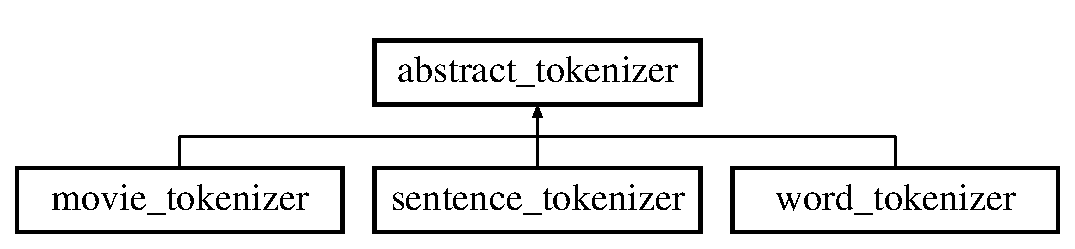
\includegraphics[height=2.000000cm]{classabstract__tokenizer}
\end{center}
\end{figure}
\subsection*{Public Member Functions}
\begin{DoxyCompactItemize}
\item 
\mbox{\Hypertarget{classabstract__tokenizer_a03902af3bbdd717811b3eb56c9fc0060}\label{classabstract__tokenizer_a03902af3bbdd717811b3eb56c9fc0060}} 
\hyperlink{classabstract__tokenizer_a03902af3bbdd717811b3eb56c9fc0060}{abstract\+\_\+tokenizer} ()
\begin{DoxyCompactList}\small\item\em A default constructor. \end{DoxyCompactList}\item 
\mbox{\Hypertarget{classabstract__tokenizer_aa68856356e49784c7d0eed48d24f8738}\label{classabstract__tokenizer_aa68856356e49784c7d0eed48d24f8738}} 
virtual \hyperlink{classabstract__tokenizer_aa68856356e49784c7d0eed48d24f8738}{$\sim$abstract\+\_\+tokenizer} ()
\begin{DoxyCompactList}\small\item\em A virtual destructor. \end{DoxyCompactList}\end{DoxyCompactItemize}


The documentation for this class was generated from the following files\+:\begin{DoxyCompactItemize}
\item 
abstract\+\_\+tokenizer.\+h\item 
abstract\+\_\+tokenizer.\+cpp\end{DoxyCompactItemize}

\hypertarget{classdocument}{}\section{document Class Reference}
\label{classdocument}\index{document@{document}}
Inheritance diagram for document\+:\begin{figure}[H]
\begin{center}
\leavevmode
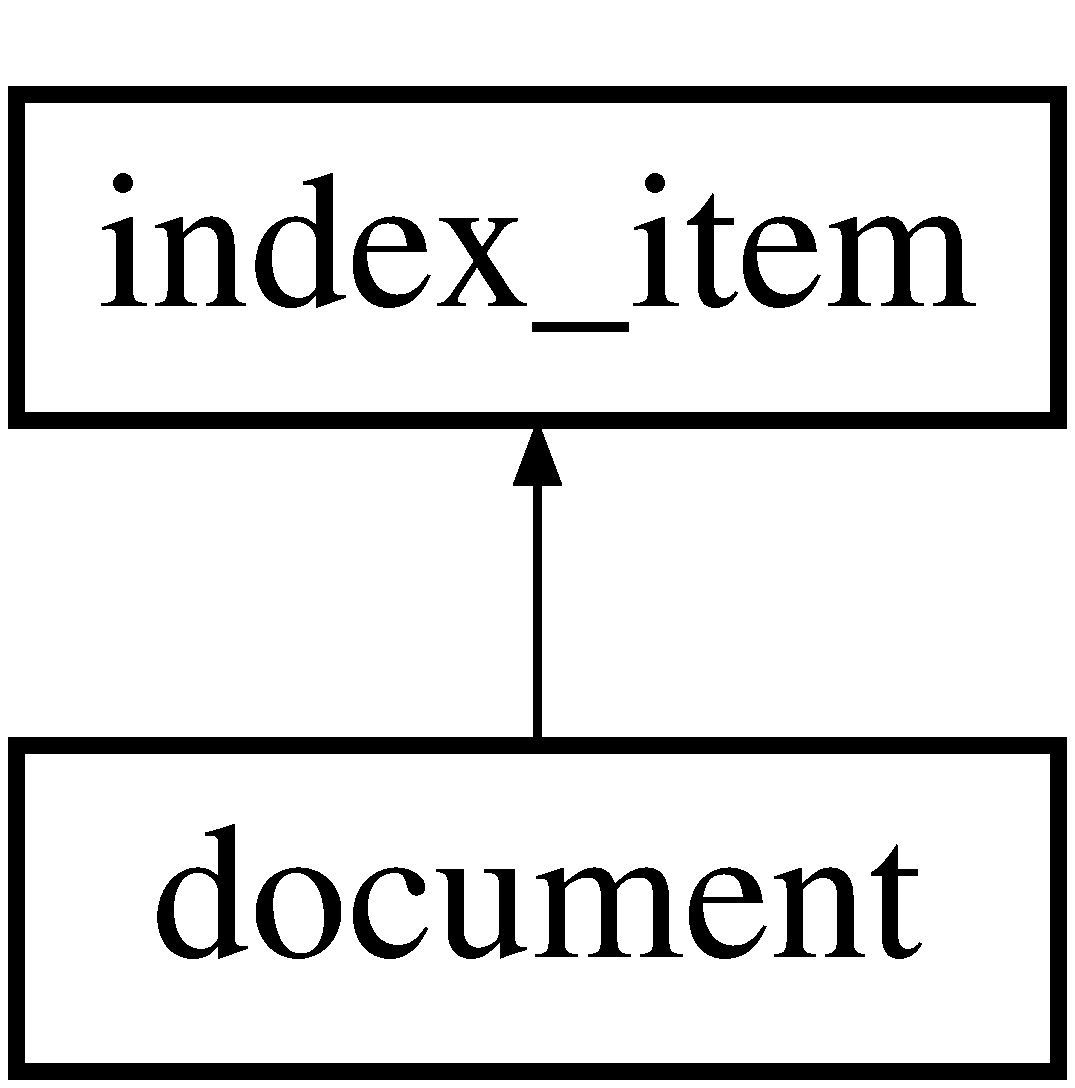
\includegraphics[height=2.000000cm]{classdocument}
\end{center}
\end{figure}
\subsection*{Public Member Functions}
\begin{DoxyCompactItemize}
\item 
\hyperlink{classdocument_af1a85718219b8da6f1befaac0bf87989}{document} ()
\begin{DoxyCompactList}\small\item\em A default constructor. \end{DoxyCompactList}\item 
\mbox{\Hypertarget{classdocument_afff6a78ede7767d8cbc0cb4566ae64da}\label{classdocument_afff6a78ede7767d8cbc0cb4566ae64da}} 
\hyperlink{classdocument_afff6a78ede7767d8cbc0cb4566ae64da}{$\sim$document} ()
\begin{DoxyCompactList}\small\item\em A default destructor. \end{DoxyCompactList}\item 
\hyperlink{classdocument_af8e0d4d3a3eeeac31022ebe0e76c5571}{document} (string \hyperlink{classdocument_a19e6fd5bb89537dc566df2eac658e5a6}{name}, int num)
\begin{DoxyCompactList}\small\item\em Another constructor. \end{DoxyCompactList}\item 
string \hyperlink{classdocument_a19e6fd5bb89537dc566df2eac658e5a6}{name} () const
\begin{DoxyCompactList}\small\item\em An accessor for the document\textquotesingle{}s name. \end{DoxyCompactList}\item 
int \hyperlink{classdocument_ac8755191462341296e2be04db6f8f4e5}{get\+Doc\+Num} () const
\begin{DoxyCompactList}\small\item\em An accessor for the document\textquotesingle{}s number. \end{DoxyCompactList}\end{DoxyCompactItemize}
\subsection*{Friends}
\begin{DoxyCompactItemize}
\item 
ostream \& \hyperlink{classdocument_aafdf2f4ecb817252c0e22f7c072ec5b0}{operator$<$$<$} (ostream \&os, \hyperlink{classdocument}{document} \&d)
\begin{DoxyCompactList}\small\item\em A friend operator$<$$<$ overload. \end{DoxyCompactList}\end{DoxyCompactItemize}
\subsection*{Additional Inherited Members}


\subsection{Constructor \& Destructor Documentation}
\mbox{\Hypertarget{classdocument_af1a85718219b8da6f1befaac0bf87989}\label{classdocument_af1a85718219b8da6f1befaac0bf87989}} 
\index{document@{document}!document@{document}}
\index{document@{document}!document@{document}}
\subsubsection{\texorpdfstring{document()}{document()}\hspace{0.1cm}{\footnotesize\ttfamily [1/2]}}
{\footnotesize\ttfamily document\+::document (\begin{DoxyParamCaption}{ }\end{DoxyParamCaption})}



A default constructor. 

The default constructor sets the filename and content to \char`\"{}\char`\"{}, and the size to 0 \mbox{\Hypertarget{classdocument_af8e0d4d3a3eeeac31022ebe0e76c5571}\label{classdocument_af8e0d4d3a3eeeac31022ebe0e76c5571}} 
\index{document@{document}!document@{document}}
\index{document@{document}!document@{document}}
\subsubsection{\texorpdfstring{document()}{document()}\hspace{0.1cm}{\footnotesize\ttfamily [2/2]}}
{\footnotesize\ttfamily document\+::document (\begin{DoxyParamCaption}\item[{string}]{name,  }\item[{int}]{num }\end{DoxyParamCaption})}



Another constructor. 


\begin{DoxyParams}{Parameters}
{\em filename} & filename of the document to be constructed. \\
\hline
{\em num} & doc\+Num of the document to be constructed.\\
\hline
\end{DoxyParams}
The constructor takes a string name, and sets the document\textquotesingle{}s name as that string It then creates a filestream with the string name, and reads its contents into the document\textquotesingle{}s content field It then sets the document\textquotesingle{}s size to the size of content 

\subsection{Member Function Documentation}
\mbox{\Hypertarget{classdocument_ac8755191462341296e2be04db6f8f4e5}\label{classdocument_ac8755191462341296e2be04db6f8f4e5}} 
\index{document@{document}!get\+Doc\+Num@{get\+Doc\+Num}}
\index{get\+Doc\+Num@{get\+Doc\+Num}!document@{document}}
\subsubsection{\texorpdfstring{get\+Doc\+Num()}{getDocNum()}}
{\footnotesize\ttfamily int document\+::get\+Doc\+Num (\begin{DoxyParamCaption}{ }\end{DoxyParamCaption}) const}



An accessor for the document\textquotesingle{}s number. 

\begin{DoxyReturn}{Returns}
An int\+: doc\+Num of the document.
\end{DoxyReturn}
This accessor returns the document\textquotesingle{}s filename \mbox{\Hypertarget{classdocument_a19e6fd5bb89537dc566df2eac658e5a6}\label{classdocument_a19e6fd5bb89537dc566df2eac658e5a6}} 
\index{document@{document}!name@{name}}
\index{name@{name}!document@{document}}
\subsubsection{\texorpdfstring{name()}{name()}}
{\footnotesize\ttfamily string document\+::name (\begin{DoxyParamCaption}{ }\end{DoxyParamCaption}) const}



An accessor for the document\textquotesingle{}s name. 

\begin{DoxyReturn}{Returns}
A string\+: name of the document.
\end{DoxyReturn}
This accessor returns the document\textquotesingle{}s filename 

\subsection{Friends And Related Function Documentation}
\mbox{\Hypertarget{classdocument_aafdf2f4ecb817252c0e22f7c072ec5b0}\label{classdocument_aafdf2f4ecb817252c0e22f7c072ec5b0}} 
\index{document@{document}!operator$<$$<$@{operator$<$$<$}}
\index{operator$<$$<$@{operator$<$$<$}!document@{document}}
\subsubsection{\texorpdfstring{operator$<$$<$}{operator<<}}
{\footnotesize\ttfamily ostream\& operator$<$$<$ (\begin{DoxyParamCaption}\item[{ostream \&}]{os,  }\item[{\hyperlink{classdocument}{document} \&}]{d }\end{DoxyParamCaption})\hspace{0.3cm}{\ttfamily [friend]}}



A friend operator$<$$<$ overload. 

Puts document\textquotesingle{}s information into an ostream 
\begin{DoxyParams}{Parameters}
{\em os} & the ostream into which we put document information \\
\hline
{\em d} & the document which\textquotesingle{}s information we print out \\
\hline
\end{DoxyParams}
\begin{DoxyReturn}{Returns}
an ostream\+: the contents of document
\end{DoxyReturn}
This method overloads the operator$<$$<$ It reads the file\textquotesingle{}s information into the ostream 

The documentation for this class was generated from the following files\+:\begin{DoxyCompactItemize}
\item 
document.\+h\item 
document.\+cpp\end{DoxyCompactItemize}

\hypertarget{classdocument__indexer}{}\section{document\+\_\+indexer Class Reference}
\label{classdocument__indexer}\index{document\+\_\+indexer@{document\+\_\+indexer}}
Inheritance diagram for document\+\_\+indexer\+:\begin{figure}[H]
\begin{center}
\leavevmode
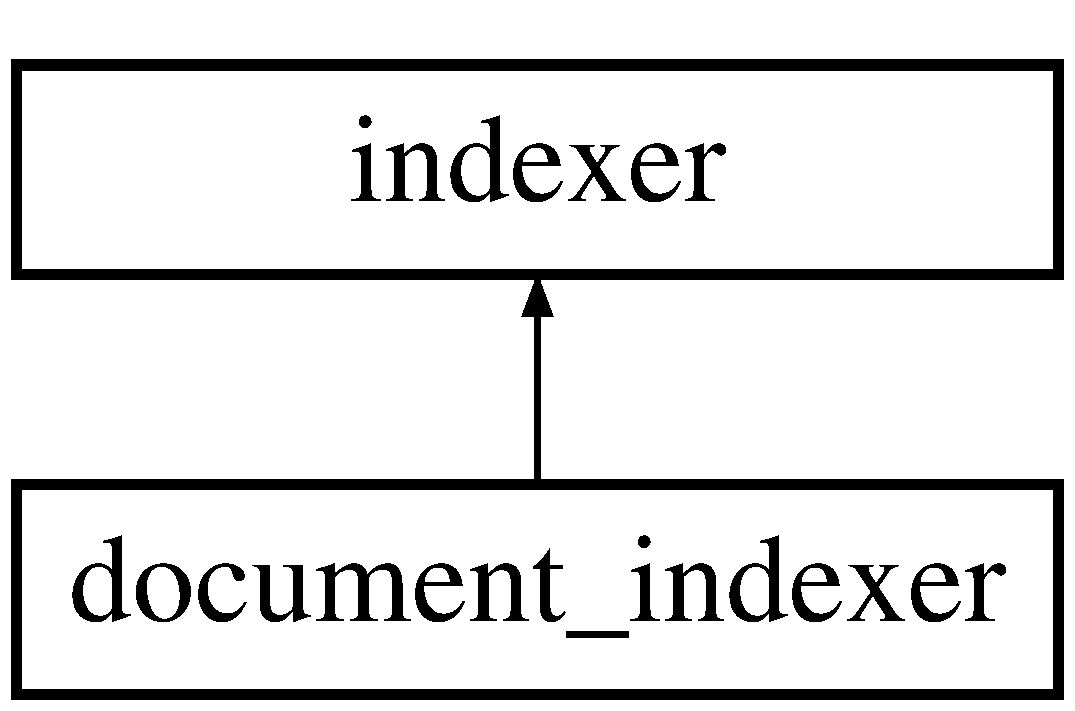
\includegraphics[height=2.000000cm]{classdocument__indexer}
\end{center}
\end{figure}
\subsection*{Public Member Functions}
\begin{DoxyCompactItemize}
\item 
\hyperlink{classdocument__indexer_a569b5a1dc381efce6ab2ab64644a7662}{document\+\_\+indexer} ()
\begin{DoxyCompactList}\small\item\em a default constructor. \end{DoxyCompactList}\item 
vector$<$ string $>$ \hyperlink{classdocument__indexer_a885c965f69ed1fcef8b4670d48182045}{get\+Document\+Names} ()
\begin{DoxyCompactList}\small\item\em gets the documents names \end{DoxyCompactList}\item 
\hyperlink{classindex__item}{index\+\_\+item} $\ast$ \hyperlink{classdocument__indexer_a2f17781feae3360c3900190b69709f0d}{operator\mbox{[}$\,$\mbox{]}} (string name)
\begin{DoxyCompactList}\small\item\em An operator\mbox{[}\mbox{]} overload. \end{DoxyCompactList}\item 
\hyperlink{classindex__item}{index\+\_\+item} $\ast$ \hyperlink{classdocument__indexer_ab6573986790793c03f05192a526d217d}{operator\mbox{[}$\,$\mbox{]}} (int n)
\begin{DoxyCompactList}\small\item\em an operator\mbox{[}\mbox{]} overload. \end{DoxyCompactList}\end{DoxyCompactItemize}
\subsection*{Friends}
\begin{DoxyCompactItemize}
\item 
ostream \& \hyperlink{classdocument__indexer_aa4cd3fa3dc189d5e7dc4b07ed98958e8}{operator$<$$<$} (ostream \&os, \hyperlink{classdocument__indexer}{document\+\_\+indexer} \&idx)
\begin{DoxyCompactList}\small\item\em an operator$<$$<$ overload \end{DoxyCompactList}\end{DoxyCompactItemize}
\subsection*{Additional Inherited Members}


\subsection{Constructor \& Destructor Documentation}
\mbox{\Hypertarget{classdocument__indexer_a569b5a1dc381efce6ab2ab64644a7662}\label{classdocument__indexer_a569b5a1dc381efce6ab2ab64644a7662}} 
\index{document\+\_\+indexer@{document\+\_\+indexer}!document\+\_\+indexer@{document\+\_\+indexer}}
\index{document\+\_\+indexer@{document\+\_\+indexer}!document\+\_\+indexer@{document\+\_\+indexer}}
\subsubsection{\texorpdfstring{document\+\_\+indexer()}{document\_indexer()}}
{\footnotesize\ttfamily document\+\_\+indexer\+::document\+\_\+indexer (\begin{DoxyParamCaption}{ }\end{DoxyParamCaption})}



a default constructor. 

Initializes the indexer\textquotesingle{}s N to 0, normalized to false, and stpw to a stopwords (\char`\"{}stopwords.\+txt\char`\"{}). 

\subsection{Member Function Documentation}
\mbox{\Hypertarget{classdocument__indexer_a885c965f69ed1fcef8b4670d48182045}\label{classdocument__indexer_a885c965f69ed1fcef8b4670d48182045}} 
\index{document\+\_\+indexer@{document\+\_\+indexer}!get\+Document\+Names@{get\+Document\+Names}}
\index{get\+Document\+Names@{get\+Document\+Names}!document\+\_\+indexer@{document\+\_\+indexer}}
\subsubsection{\texorpdfstring{get\+Document\+Names()}{getDocumentNames()}}
{\footnotesize\ttfamily vector$<$ string $>$ document\+\_\+indexer\+::get\+Document\+Names (\begin{DoxyParamCaption}{ }\end{DoxyParamCaption})}



gets the documents names 

\begin{DoxyReturn}{Returns}
the names of the documents in indexer
\end{DoxyReturn}
Iterates through all documents, and returns a vector of all names. \mbox{\Hypertarget{classdocument__indexer_a2f17781feae3360c3900190b69709f0d}\label{classdocument__indexer_a2f17781feae3360c3900190b69709f0d}} 
\index{document\+\_\+indexer@{document\+\_\+indexer}!operator\mbox{[}\mbox{]}@{operator[]}}
\index{operator\mbox{[}\mbox{]}@{operator[]}!document\+\_\+indexer@{document\+\_\+indexer}}
\subsubsection{\texorpdfstring{operator[]()}{operator[]()}\hspace{0.1cm}{\footnotesize\ttfamily [1/2]}}
{\footnotesize\ttfamily \hyperlink{classindex__item}{index\+\_\+item} $\ast$ document\+\_\+indexer\+::operator\mbox{[}$\,$\mbox{]} (\begin{DoxyParamCaption}\item[{string}]{name }\end{DoxyParamCaption})}



An operator\mbox{[}\mbox{]} overload. 


\begin{DoxyParams}{Parameters}
{\em name} & the name of the document to return \\
\hline
\end{DoxyParams}
\begin{DoxyReturn}{Returns}
the document with filename name
\end{DoxyReturn}
Iterates through all items, and returns the document with filename name \mbox{\Hypertarget{classdocument__indexer_ab6573986790793c03f05192a526d217d}\label{classdocument__indexer_ab6573986790793c03f05192a526d217d}} 
\index{document\+\_\+indexer@{document\+\_\+indexer}!operator\mbox{[}\mbox{]}@{operator[]}}
\index{operator\mbox{[}\mbox{]}@{operator[]}!document\+\_\+indexer@{document\+\_\+indexer}}
\subsubsection{\texorpdfstring{operator[]()}{operator[]()}\hspace{0.1cm}{\footnotesize\ttfamily [2/2]}}
{\footnotesize\ttfamily \hyperlink{classindex__item}{index\+\_\+item} $\ast$ document\+\_\+indexer\+::operator\mbox{[}$\,$\mbox{]} (\begin{DoxyParamCaption}\item[{int}]{n }\end{DoxyParamCaption})\hspace{0.3cm}{\ttfamily [virtual]}}



an operator\mbox{[}\mbox{]} overload. 


\begin{DoxyParams}{Parameters}
{\em n} & an int index. \\
\hline
\end{DoxyParams}
\begin{DoxyReturn}{Returns}
the document at index n.
\end{DoxyReturn}
Gets the indexer\textquotesingle{}s n\textquotesingle{}th document. 

Reimplemented from \hyperlink{classindexer_ae71041fc84d94155473de60e4407d5cc}{indexer}.



\subsection{Friends And Related Function Documentation}
\mbox{\Hypertarget{classdocument__indexer_aa4cd3fa3dc189d5e7dc4b07ed98958e8}\label{classdocument__indexer_aa4cd3fa3dc189d5e7dc4b07ed98958e8}} 
\index{document\+\_\+indexer@{document\+\_\+indexer}!operator$<$$<$@{operator$<$$<$}}
\index{operator$<$$<$@{operator$<$$<$}!document\+\_\+indexer@{document\+\_\+indexer}}
\subsubsection{\texorpdfstring{operator$<$$<$}{operator<<}}
{\footnotesize\ttfamily ostream\& operator$<$$<$ (\begin{DoxyParamCaption}\item[{ostream \&}]{os,  }\item[{\hyperlink{classdocument__indexer}{document\+\_\+indexer} \&}]{idx }\end{DoxyParamCaption})\hspace{0.3cm}{\ttfamily [friend]}}



an operator$<$$<$ overload 


\begin{DoxyParams}{Parameters}
{\em os} & the outstream which will receive the matrix information \\
\hline
{\em idx} & the indexer from which we take information \\
\hline
\end{DoxyParams}
\begin{DoxyReturn}{Returns}
the outstream with matrix information.
\end{DoxyReturn}
Fills an outstream with the document matrices information (term frequency, weight etc.) 

The documentation for this class was generated from the following files\+:\begin{DoxyCompactItemize}
\item 
document\+\_\+indexer.\+h\item 
document\+\_\+indexer.\+cpp\end{DoxyCompactItemize}

\hypertarget{classindex__exception}{}\section{index\+\_\+exception Class Reference}
\label{classindex__exception}\index{index\+\_\+exception@{index\+\_\+exception}}
Inheritance diagram for index\+\_\+exception\+:\begin{figure}[H]
\begin{center}
\leavevmode
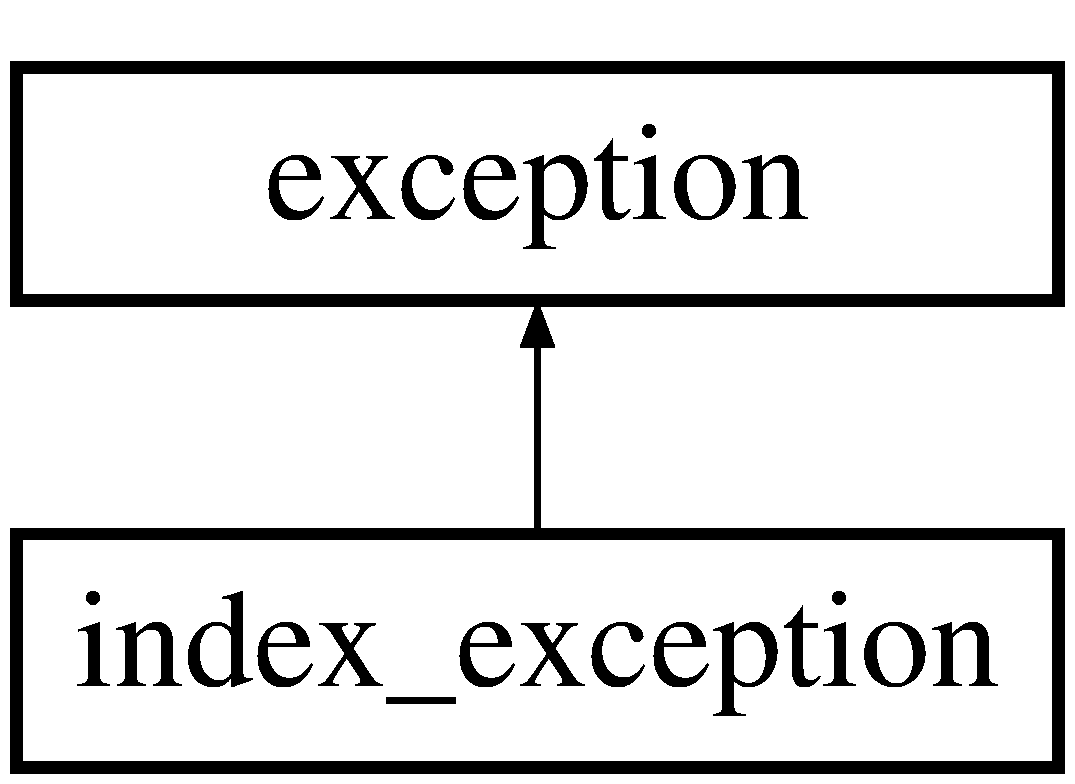
\includegraphics[height=2.000000cm]{classindex__exception}
\end{center}
\end{figure}
\subsection*{Public Member Functions}
\begin{DoxyCompactItemize}
\item 
\mbox{\Hypertarget{classindex__exception_ab802455f8559c660215559eb1fe75274}\label{classindex__exception_ab802455f8559c660215559eb1fe75274}} 
const char $\ast$ \hyperlink{classindex__exception_ab802455f8559c660215559eb1fe75274}{what} () const noexcept override
\begin{DoxyCompactList}\small\item\em Overlaading the virtual function \hyperlink{classindex__exception_ab802455f8559c660215559eb1fe75274}{what()} so that it returns the error message. \end{DoxyCompactList}\end{DoxyCompactItemize}


The documentation for this class was generated from the following files\+:\begin{DoxyCompactItemize}
\item 
index\+\_\+exception.\+h\item 
index\+\_\+exception.\+cpp\end{DoxyCompactItemize}

\hypertarget{classindex__item}{}\section{index\+\_\+item Class Reference}
\label{classindex__item}\index{index\+\_\+item@{index\+\_\+item}}
Inheritance diagram for index\+\_\+item\+:\begin{figure}[H]
\begin{center}
\leavevmode
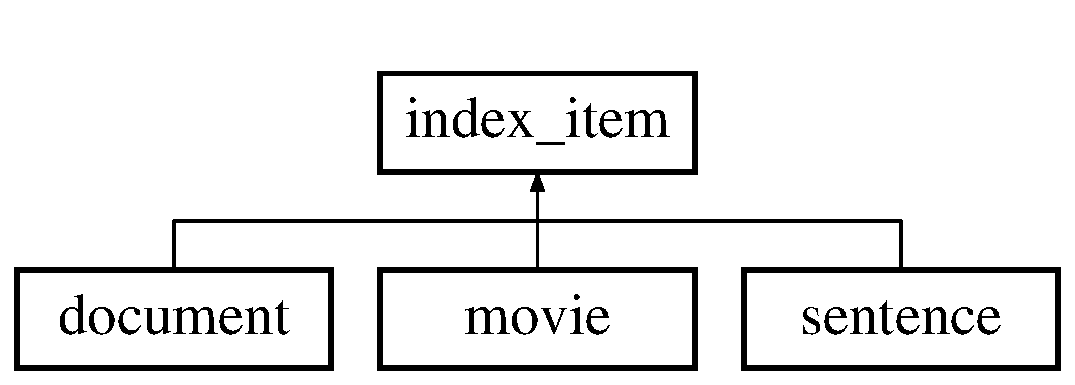
\includegraphics[height=2.000000cm]{classindex__item}
\end{center}
\end{figure}
\subsection*{Public Member Functions}
\begin{DoxyCompactItemize}
\item 
\mbox{\Hypertarget{classindex__item_a26948d7ad5975fe8160fdedb58df9904}\label{classindex__item_a26948d7ad5975fe8160fdedb58df9904}} 
\hyperlink{classindex__item_a26948d7ad5975fe8160fdedb58df9904}{index\+\_\+item} ()
\begin{DoxyCompactList}\small\item\em A default constructor. \end{DoxyCompactList}\item 
size\+\_\+t \hyperlink{classindex__item_a16fbb1fcb7c9296afd03eaed51175935}{size} () const
\begin{DoxyCompactList}\small\item\em An accessor for the item\textquotesingle{}s size. \end{DoxyCompactList}\item 
string \hyperlink{classindex__item_ae95390ac357a5e10b6c1335a49d91e83}{get\+\_\+content} () const
\begin{DoxyCompactList}\small\item\em An accessor for the item\textquotesingle{}s content. \end{DoxyCompactList}\end{DoxyCompactItemize}
\subsection*{Protected Attributes}
\begin{DoxyCompactItemize}
\item 
\mbox{\Hypertarget{classindex__item_a166149dcf6112a70a90c5d0a1742d935}\label{classindex__item_a166149dcf6112a70a90c5d0a1742d935}} 
size\+\_\+t \hyperlink{classindex__item_a166149dcf6112a70a90c5d0a1742d935}{item\+\_\+size}
\begin{DoxyCompactList}\small\item\em A private string\+: the item\textquotesingle{}s content. \end{DoxyCompactList}\item 
\mbox{\Hypertarget{classindex__item_a0bf501d53a26d87693da9ca8a038bfb7}\label{classindex__item_a0bf501d53a26d87693da9ca8a038bfb7}} 
string \hyperlink{classindex__item_a0bf501d53a26d87693da9ca8a038bfb7}{content}
\begin{DoxyCompactList}\small\item\em a private size\+\_\+t\+: the item\textquotesingle{}s size. \end{DoxyCompactList}\end{DoxyCompactItemize}


\subsection{Member Function Documentation}
\mbox{\Hypertarget{classindex__item_ae95390ac357a5e10b6c1335a49d91e83}\label{classindex__item_ae95390ac357a5e10b6c1335a49d91e83}} 
\index{index\+\_\+item@{index\+\_\+item}!get\+\_\+content@{get\+\_\+content}}
\index{get\+\_\+content@{get\+\_\+content}!index\+\_\+item@{index\+\_\+item}}
\subsubsection{\texorpdfstring{get\+\_\+content()}{get\_content()}}
{\footnotesize\ttfamily string index\+\_\+item\+::get\+\_\+content (\begin{DoxyParamCaption}{ }\end{DoxyParamCaption}) const}



An accessor for the item\textquotesingle{}s content. 

\begin{DoxyReturn}{Returns}
A string\+: the content of the item.
\end{DoxyReturn}
This accessor returns the document\textquotesingle{}s content \mbox{\Hypertarget{classindex__item_a16fbb1fcb7c9296afd03eaed51175935}\label{classindex__item_a16fbb1fcb7c9296afd03eaed51175935}} 
\index{index\+\_\+item@{index\+\_\+item}!size@{size}}
\index{size@{size}!index\+\_\+item@{index\+\_\+item}}
\subsubsection{\texorpdfstring{size()}{size()}}
{\footnotesize\ttfamily size\+\_\+t index\+\_\+item\+::size (\begin{DoxyParamCaption}{ }\end{DoxyParamCaption}) const}



An accessor for the item\textquotesingle{}s size. 

\begin{DoxyReturn}{Returns}
A size\+\_\+t\+: the size of the item.
\end{DoxyReturn}
This accessor returns the document\textquotesingle{}s size 

The documentation for this class was generated from the following files\+:\begin{DoxyCompactItemize}
\item 
index\+\_\+item.\+h\item 
index\+\_\+item.\+cpp\end{DoxyCompactItemize}

\hypertarget{classindexer}{}\section{indexer Class Reference}
\label{classindexer}\index{indexer@{indexer}}
Inheritance diagram for indexer\+:\begin{figure}[H]
\begin{center}
\leavevmode
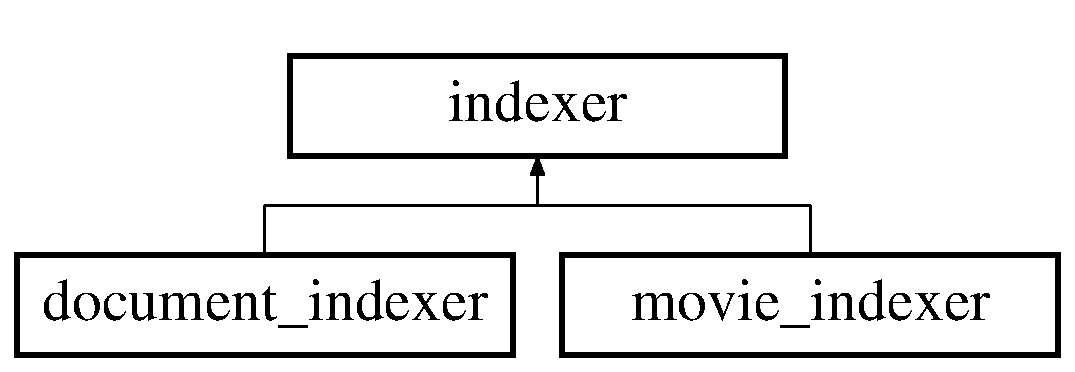
\includegraphics[height=2.000000cm]{classindexer}
\end{center}
\end{figure}
\subsection*{Public Types}
\begin{DoxyCompactItemize}
\item 
\mbox{\Hypertarget{classindexer_aeadc68a96ef7492b4d320eaf470fb5f6}\label{classindexer_aeadc68a96ef7492b4d320eaf470fb5f6}} 
enum \hyperlink{classindexer_aeadc68a96ef7492b4d320eaf470fb5f6}{Exceptions} \{ {\bfseries I\+N\+D\+E\+X\+\_\+\+N\+O\+T\+\_\+\+N\+O\+R\+M\+A\+L\+I\+Z\+ED}
 \}\begin{DoxyCompactList}\small\item\em an exception to be thrown when attemptin to query an un-\/normalized indexer. \end{DoxyCompactList}
\end{DoxyCompactItemize}
\subsection*{Public Member Functions}
\begin{DoxyCompactItemize}
\item 
\hyperlink{classindexer_acbbcbad080a7ae43ed78840fcf006960}{indexer} ()
\begin{DoxyCompactList}\small\item\em a default constructor. \end{DoxyCompactList}\item 
int \hyperlink{classindexer_ad9e5eee599f4677d7a6cca2f53aeec44}{get\+Size} ()
\begin{DoxyCompactList}\small\item\em an accessor for size. \end{DoxyCompactList}\item 
bool \hyperlink{classindexer_a48c05d99699e2191d606936b35ecbb0d}{is\+Normalize} ()
\begin{DoxyCompactList}\small\item\em an accessor for normalize. \end{DoxyCompactList}\item 
\hyperlink{classstopwords}{stopwords} $\ast$ \hyperlink{classindexer_a78be8aabef768ba82208956e53316cc5}{getstpw} ()
\begin{DoxyCompactList}\small\item\em an accessor for stpw. \end{DoxyCompactList}\item 
vector$<$ \hyperlink{classindex__item}{index\+\_\+item} $\ast$ $>$ \& \hyperlink{classindexer_ad576259a08d87b8d4486793522a0ca5a}{get\+Items} ()
\begin{DoxyCompactList}\small\item\em an accessor for documents. \end{DoxyCompactList}\item 
map$<$ string, int $>$ \& \hyperlink{classindexer_a99c8633ff92270ecbe76a5c9cf57e2e0}{get\+Dft} ()
\begin{DoxyCompactList}\small\item\em an accessor for dft. \end{DoxyCompactList}\item 
map$<$ string, map$<$ \hyperlink{classindex__item}{index\+\_\+item} $\ast$, int $>$ $>$ \& \hyperlink{classindexer_ad2afffef1c97feb0c7934951ce35319c}{get\+T\+Ftd1} ()
\begin{DoxyCompactList}\small\item\em an accessor for tftd1. \end{DoxyCompactList}\item 
map$<$ string, map$<$ \hyperlink{classindex__item}{index\+\_\+item} $\ast$, int $>$ $>$ \& \hyperlink{classindexer_ab819d6ad0ae7fb00254a5d41f4cc92cd}{get\+T\+Ftd2} ()
\begin{DoxyCompactList}\small\item\em an accessor for tftd2. \end{DoxyCompactList}\item 
map$<$ string, map$<$ \hyperlink{classindex__item}{index\+\_\+item} $\ast$, double $>$ $>$ \& \hyperlink{classindexer_a8c9a0dadc14a83bdfa36c8b7555cbc6c}{get\+Wtd} ()
\begin{DoxyCompactList}\small\item\em an accessor for wtd. \end{DoxyCompactList}\item 
map$<$ \hyperlink{classindex__item}{index\+\_\+item} $\ast$, int $>$ \& \hyperlink{classindexer_a8886ee24d98c5129a6582a95f65e31f6}{get\+Total1} ()
\begin{DoxyCompactList}\small\item\em an accessor for total1. \end{DoxyCompactList}\item 
map$<$ \hyperlink{classindex__item}{index\+\_\+item} $\ast$, int $>$ \& \hyperlink{classindexer_a8717246599f696d38d2b7051071b8957}{get\+Total2} ()
\begin{DoxyCompactList}\small\item\em an accessor for total2. \end{DoxyCompactList}\item 
void \hyperlink{classindexer_afd19e249c5224de7b4b308c5420f2412}{normalize} ()
\begin{DoxyCompactList}\small\item\em a function which normalizes the indexer. \end{DoxyCompactList}\item 
virtual \hyperlink{classindex__item}{index\+\_\+item} $\ast$ \hyperlink{classindexer_ae71041fc84d94155473de60e4407d5cc}{operator\mbox{[}$\,$\mbox{]}} (int n)
\begin{DoxyCompactList}\small\item\em an operator\mbox{[}\mbox{]} overload. \end{DoxyCompactList}\end{DoxyCompactItemize}
\subsection*{Protected Attributes}
\begin{DoxyCompactItemize}
\item 
\mbox{\Hypertarget{classindexer_a0742c29a845289118c3f4b75653be72c}\label{classindexer_a0742c29a845289118c3f4b75653be72c}} 
int \hyperlink{classindexer_a0742c29a845289118c3f4b75653be72c}{N}
\begin{DoxyCompactList}\small\item\em A private int\+: the number of index items. \end{DoxyCompactList}\item 
\mbox{\Hypertarget{classindexer_a8c6e10131bfdffba3d221076176a16c7}\label{classindexer_a8c6e10131bfdffba3d221076176a16c7}} 
bool \hyperlink{classindexer_a8c6e10131bfdffba3d221076176a16c7}{normalized}
\begin{DoxyCompactList}\small\item\em a private boolean\+: whether the indexer has been normalized. \end{DoxyCompactList}\item 
\mbox{\Hypertarget{classindexer_a627b020657c54f3c2ba35953311bf2b2}\label{classindexer_a627b020657c54f3c2ba35953311bf2b2}} 
\hyperlink{classstopwords}{stopwords} $\ast$ \hyperlink{classindexer_a627b020657c54f3c2ba35953311bf2b2}{stpw}
\begin{DoxyCompactList}\small\item\em a private stopwords\+: the stopwords the indexer should keep track of. \end{DoxyCompactList}\item 
\mbox{\Hypertarget{classindexer_a3b00610add9f8f127eb1c1a22e8d7886}\label{classindexer_a3b00610add9f8f127eb1c1a22e8d7886}} 
vector$<$ \hyperlink{classindex__item}{index\+\_\+item} $\ast$ $>$ \hyperlink{classindexer_a3b00610add9f8f127eb1c1a22e8d7886}{items}
\begin{DoxyCompactList}\small\item\em a private vector of documents\+: the list of documents which\textquotesingle{}s score the indexer should keep. \end{DoxyCompactList}\item 
\mbox{\Hypertarget{classindexer_a4de4c0d5adaa7b61ccd81e83ecef5de0}\label{classindexer_a4de4c0d5adaa7b61ccd81e83ecef5de0}} 
map$<$ string, int $>$ \hyperlink{classindexer_a4de4c0d5adaa7b61ccd81e83ecef5de0}{dft}
\begin{DoxyCompactList}\small\item\em a private map of string, int\+: the total number of documents that a token appears in. (Document Frequency) \end{DoxyCompactList}\item 
\mbox{\Hypertarget{classindexer_a0139107164efd7e1d8ee95680a8f623e}\label{classindexer_a0139107164efd7e1d8ee95680a8f623e}} 
map$<$ string, map$<$ \hyperlink{classindex__item}{index\+\_\+item} $\ast$, int $>$ $>$ \hyperlink{classindexer_a0139107164efd7e1d8ee95680a8f623e}{tftd1}
\begin{DoxyCompactList}\small\item\em a private map of string, pair$<$string, int$>$ vector\+: the token frequency in documents. The pair is document name -\/ weight in that document \end{DoxyCompactList}\item 
\mbox{\Hypertarget{classindexer_a1ff1c5347d49058577a4426c566fa869}\label{classindexer_a1ff1c5347d49058577a4426c566fa869}} 
map$<$ string, map$<$ \hyperlink{classindex__item}{index\+\_\+item} $\ast$, int $>$ $>$ \hyperlink{classindexer_a1ff1c5347d49058577a4426c566fa869}{tftd2}
\begin{DoxyCompactList}\small\item\em a private map of string, pair$<$string, int$>$ vector\+: The same as tftd1, but with stopwords removed. \end{DoxyCompactList}\item 
\mbox{\Hypertarget{classindexer_a74d1cf4b9a28f2772334d2abadab014d}\label{classindexer_a74d1cf4b9a28f2772334d2abadab014d}} 
map$<$ string, map$<$ \hyperlink{classindex__item}{index\+\_\+item} $\ast$, double $>$ $>$ \hyperlink{classindexer_a74d1cf4b9a28f2772334d2abadab014d}{wtd}
\begin{DoxyCompactList}\small\item\em a private map of string, pair$<$string, double$>$ vector\+: the weight of each token in each document, stored similarly to tftd1 but for weight instead of frequency. \end{DoxyCompactList}\item 
\mbox{\Hypertarget{classindexer_aa8fe5fc7623db3c099e9d1604ffa09bb}\label{classindexer_aa8fe5fc7623db3c099e9d1604ffa09bb}} 
map$<$ \hyperlink{classindex__item}{index\+\_\+item} $\ast$, int $>$ \hyperlink{classindexer_aa8fe5fc7623db3c099e9d1604ffa09bb}{total1}
\begin{DoxyCompactList}\small\item\em a private pair vector\+: the total number of words per document, stored similarly to the weight in tftd1. \end{DoxyCompactList}\item 
\mbox{\Hypertarget{classindexer_a5b4ef5367c4d3f0f35b96c180c67e989}\label{classindexer_a5b4ef5367c4d3f0f35b96c180c67e989}} 
map$<$ \hyperlink{classindex__item}{index\+\_\+item} $\ast$, int $>$ \hyperlink{classindexer_a5b4ef5367c4d3f0f35b96c180c67e989}{total2}
\begin{DoxyCompactList}\small\item\em a private pair vector\+: the same as total1, but without stopwords. \end{DoxyCompactList}\end{DoxyCompactItemize}
\subsection*{Friends}
\begin{DoxyCompactItemize}
\item 
\hyperlink{classindex__item}{index\+\_\+item} \& \hyperlink{classindexer_af6526a689e8ed16f67708180a988b8d8}{operator$>$$>$} (\hyperlink{classindex__item}{index\+\_\+item} $\ast$d, \hyperlink{classindexer}{indexer} \&idx)
\begin{DoxyCompactList}\small\item\em an operator$>$$>$ overload. \end{DoxyCompactList}\end{DoxyCompactItemize}


\subsection{Constructor \& Destructor Documentation}
\mbox{\Hypertarget{classindexer_acbbcbad080a7ae43ed78840fcf006960}\label{classindexer_acbbcbad080a7ae43ed78840fcf006960}} 
\index{indexer@{indexer}!indexer@{indexer}}
\index{indexer@{indexer}!indexer@{indexer}}
\subsubsection{\texorpdfstring{indexer()}{indexer()}}
{\footnotesize\ttfamily indexer\+::indexer (\begin{DoxyParamCaption}{ }\end{DoxyParamCaption})}



a default constructor. 

Initializes the indexer\textquotesingle{}s N to 0, normalized to false, and stpw to a stopwords (\char`\"{}stopwords.\+txt\char`\"{}). 

\subsection{Member Function Documentation}
\mbox{\Hypertarget{classindexer_a99c8633ff92270ecbe76a5c9cf57e2e0}\label{classindexer_a99c8633ff92270ecbe76a5c9cf57e2e0}} 
\index{indexer@{indexer}!get\+Dft@{get\+Dft}}
\index{get\+Dft@{get\+Dft}!indexer@{indexer}}
\subsubsection{\texorpdfstring{get\+Dft()}{getDft()}}
{\footnotesize\ttfamily map$<$ string, int $>$ \& indexer\+::get\+Dft (\begin{DoxyParamCaption}{ }\end{DoxyParamCaption})}



an accessor for dft. 

\begin{DoxyReturn}{Returns}
the dft of indexer. 
\end{DoxyReturn}
\mbox{\Hypertarget{classindexer_ad576259a08d87b8d4486793522a0ca5a}\label{classindexer_ad576259a08d87b8d4486793522a0ca5a}} 
\index{indexer@{indexer}!get\+Items@{get\+Items}}
\index{get\+Items@{get\+Items}!indexer@{indexer}}
\subsubsection{\texorpdfstring{get\+Items()}{getItems()}}
{\footnotesize\ttfamily vector$<$ \hyperlink{classindex__item}{index\+\_\+item} $\ast$ $>$ \& indexer\+::get\+Items (\begin{DoxyParamCaption}{ }\end{DoxyParamCaption})}



an accessor for documents. 

\begin{DoxyReturn}{Returns}
the documents in indexer. 
\end{DoxyReturn}
\mbox{\Hypertarget{classindexer_ad9e5eee599f4677d7a6cca2f53aeec44}\label{classindexer_ad9e5eee599f4677d7a6cca2f53aeec44}} 
\index{indexer@{indexer}!get\+Size@{get\+Size}}
\index{get\+Size@{get\+Size}!indexer@{indexer}}
\subsubsection{\texorpdfstring{get\+Size()}{getSize()}}
{\footnotesize\ttfamily int indexer\+::get\+Size (\begin{DoxyParamCaption}{ }\end{DoxyParamCaption})}



an accessor for size. 

\begin{DoxyReturn}{Returns}
the size of the indexer.
\end{DoxyReturn}
a function to return the size of the indexer \mbox{\Hypertarget{classindexer_a78be8aabef768ba82208956e53316cc5}\label{classindexer_a78be8aabef768ba82208956e53316cc5}} 
\index{indexer@{indexer}!getstpw@{getstpw}}
\index{getstpw@{getstpw}!indexer@{indexer}}
\subsubsection{\texorpdfstring{getstpw()}{getstpw()}}
{\footnotesize\ttfamily \hyperlink{classstopwords}{stopwords} $\ast$ indexer\+::getstpw (\begin{DoxyParamCaption}{ }\end{DoxyParamCaption})}



an accessor for stpw. 

\begin{DoxyReturn}{Returns}
the indexer\textquotesingle{}s stopwords. 
\end{DoxyReturn}
\mbox{\Hypertarget{classindexer_ad2afffef1c97feb0c7934951ce35319c}\label{classindexer_ad2afffef1c97feb0c7934951ce35319c}} 
\index{indexer@{indexer}!get\+T\+Ftd1@{get\+T\+Ftd1}}
\index{get\+T\+Ftd1@{get\+T\+Ftd1}!indexer@{indexer}}
\subsubsection{\texorpdfstring{get\+T\+Ftd1()}{getTFtd1()}}
{\footnotesize\ttfamily map$<$ string, map$<$ \hyperlink{classindex__item}{index\+\_\+item} $\ast$, int $>$ $>$ \& indexer\+::get\+T\+Ftd1 (\begin{DoxyParamCaption}{ }\end{DoxyParamCaption})}



an accessor for tftd1. 

\begin{DoxyReturn}{Returns}
the indexer\textquotesingle{}s tftd1. 
\end{DoxyReturn}
\mbox{\Hypertarget{classindexer_ab819d6ad0ae7fb00254a5d41f4cc92cd}\label{classindexer_ab819d6ad0ae7fb00254a5d41f4cc92cd}} 
\index{indexer@{indexer}!get\+T\+Ftd2@{get\+T\+Ftd2}}
\index{get\+T\+Ftd2@{get\+T\+Ftd2}!indexer@{indexer}}
\subsubsection{\texorpdfstring{get\+T\+Ftd2()}{getTFtd2()}}
{\footnotesize\ttfamily map$<$ string, map$<$ \hyperlink{classindex__item}{index\+\_\+item} $\ast$, int $>$ $>$ \& indexer\+::get\+T\+Ftd2 (\begin{DoxyParamCaption}{ }\end{DoxyParamCaption})}



an accessor for tftd2. 

\begin{DoxyReturn}{Returns}
the indexer\textquotesingle{}s tftd2. 
\end{DoxyReturn}
\mbox{\Hypertarget{classindexer_a8886ee24d98c5129a6582a95f65e31f6}\label{classindexer_a8886ee24d98c5129a6582a95f65e31f6}} 
\index{indexer@{indexer}!get\+Total1@{get\+Total1}}
\index{get\+Total1@{get\+Total1}!indexer@{indexer}}
\subsubsection{\texorpdfstring{get\+Total1()}{getTotal1()}}
{\footnotesize\ttfamily map$<$ \hyperlink{classindex__item}{index\+\_\+item} $\ast$, int $>$ \& indexer\+::get\+Total1 (\begin{DoxyParamCaption}{ }\end{DoxyParamCaption})}



an accessor for total1. 

\begin{DoxyReturn}{Returns}
the indexer\textquotesingle{}s total1. 
\end{DoxyReturn}
\mbox{\Hypertarget{classindexer_a8717246599f696d38d2b7051071b8957}\label{classindexer_a8717246599f696d38d2b7051071b8957}} 
\index{indexer@{indexer}!get\+Total2@{get\+Total2}}
\index{get\+Total2@{get\+Total2}!indexer@{indexer}}
\subsubsection{\texorpdfstring{get\+Total2()}{getTotal2()}}
{\footnotesize\ttfamily map$<$ \hyperlink{classindex__item}{index\+\_\+item} $\ast$, int $>$ \& indexer\+::get\+Total2 (\begin{DoxyParamCaption}{ }\end{DoxyParamCaption})}



an accessor for total2. 

\begin{DoxyReturn}{Returns}
the indexer\textquotesingle{}s total2. 
\end{DoxyReturn}
\mbox{\Hypertarget{classindexer_a8c9a0dadc14a83bdfa36c8b7555cbc6c}\label{classindexer_a8c9a0dadc14a83bdfa36c8b7555cbc6c}} 
\index{indexer@{indexer}!get\+Wtd@{get\+Wtd}}
\index{get\+Wtd@{get\+Wtd}!indexer@{indexer}}
\subsubsection{\texorpdfstring{get\+Wtd()}{getWtd()}}
{\footnotesize\ttfamily map$<$ string, map$<$ \hyperlink{classindex__item}{index\+\_\+item} $\ast$, double $>$ $>$ \& indexer\+::get\+Wtd (\begin{DoxyParamCaption}{ }\end{DoxyParamCaption})}



an accessor for wtd. 

\begin{DoxyReturn}{Returns}
the indexer\textquotesingle{}s wtd. 
\end{DoxyReturn}
\mbox{\Hypertarget{classindexer_a48c05d99699e2191d606936b35ecbb0d}\label{classindexer_a48c05d99699e2191d606936b35ecbb0d}} 
\index{indexer@{indexer}!is\+Normalize@{is\+Normalize}}
\index{is\+Normalize@{is\+Normalize}!indexer@{indexer}}
\subsubsection{\texorpdfstring{is\+Normalize()}{isNormalize()}}
{\footnotesize\ttfamily bool indexer\+::is\+Normalize (\begin{DoxyParamCaption}{ }\end{DoxyParamCaption})}



an accessor for normalize. 

\begin{DoxyReturn}{Returns}
if the indexer is normalized.
\end{DoxyReturn}
Checks if the indexer is normalized \mbox{\Hypertarget{classindexer_afd19e249c5224de7b4b308c5420f2412}\label{classindexer_afd19e249c5224de7b4b308c5420f2412}} 
\index{indexer@{indexer}!normalize@{normalize}}
\index{normalize@{normalize}!indexer@{indexer}}
\subsubsection{\texorpdfstring{normalize()}{normalize()}}
{\footnotesize\ttfamily void indexer\+::normalize (\begin{DoxyParamCaption}{ }\end{DoxyParamCaption})}



a function which normalizes the indexer. 

Calculates the frequency of a token (how many documents it appears in). Then, calculates the weight of a token in each document. \mbox{\Hypertarget{classindexer_ae71041fc84d94155473de60e4407d5cc}\label{classindexer_ae71041fc84d94155473de60e4407d5cc}} 
\index{indexer@{indexer}!operator\mbox{[}\mbox{]}@{operator[]}}
\index{operator\mbox{[}\mbox{]}@{operator[]}!indexer@{indexer}}
\subsubsection{\texorpdfstring{operator[]()}{operator[]()}}
{\footnotesize\ttfamily \hyperlink{classindex__item}{index\+\_\+item} $\ast$ indexer\+::operator\mbox{[}$\,$\mbox{]} (\begin{DoxyParamCaption}\item[{int}]{n }\end{DoxyParamCaption})\hspace{0.3cm}{\ttfamily [virtual]}}



an operator\mbox{[}\mbox{]} overload. 


\begin{DoxyParams}{Parameters}
{\em n} & an int index. \\
\hline
\end{DoxyParams}
\begin{DoxyReturn}{Returns}
the document at index n.
\end{DoxyReturn}
Gets the indexer\textquotesingle{}s n\textquotesingle{}th document. 

Reimplemented in \hyperlink{classdocument__indexer_ab6573986790793c03f05192a526d217d}{document\+\_\+indexer}, and \hyperlink{classmovie__indexer_aeaadd1ac660403a0f55122c6afea3acc}{movie\+\_\+indexer}.



\subsection{Friends And Related Function Documentation}
\mbox{\Hypertarget{classindexer_af6526a689e8ed16f67708180a988b8d8}\label{classindexer_af6526a689e8ed16f67708180a988b8d8}} 
\index{indexer@{indexer}!operator$>$$>$@{operator$>$$>$}}
\index{operator$>$$>$@{operator$>$$>$}!indexer@{indexer}}
\subsubsection{\texorpdfstring{operator$>$$>$}{operator>>}}
{\footnotesize\ttfamily \hyperlink{classindex__item}{index\+\_\+item}\& operator$>$$>$ (\begin{DoxyParamCaption}\item[{\hyperlink{classindex__item}{index\+\_\+item} $\ast$}]{d,  }\item[{\hyperlink{classindexer}{indexer} \&}]{idx }\end{DoxyParamCaption})\hspace{0.3cm}{\ttfamily [friend]}}



an operator$>$$>$ overload. 


\begin{DoxyParams}{Parameters}
{\em d} & the document to add to the indexer. \\
\hline
{\em idx} & the indexer to which we are adding a document. \\
\hline
\end{DoxyParams}
\begin{DoxyReturn}{Returns}
the document d.
\end{DoxyReturn}
Adds a new document to the indexer, then calculates term frequency for that document and normalizes the indexer. 

The documentation for this class was generated from the following files\+:\begin{DoxyCompactItemize}
\item 
indexer.\+h\item 
indexer.\+cpp\end{DoxyCompactItemize}

\hypertarget{classmovie}{}\section{movie Class Reference}
\label{classmovie}\index{movie@{movie}}
Inheritance diagram for movie\+:\begin{figure}[H]
\begin{center}
\leavevmode
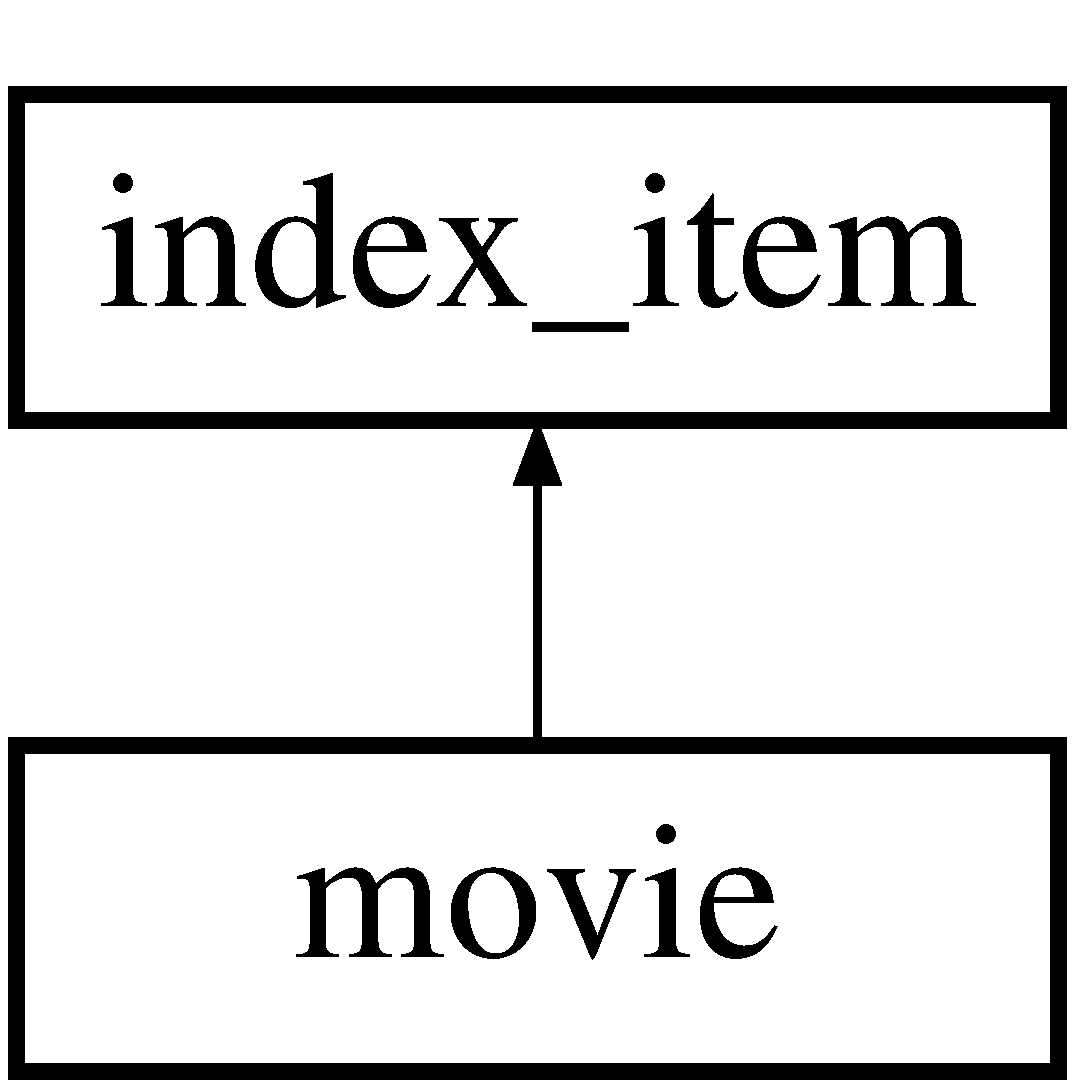
\includegraphics[height=2.000000cm]{classmovie}
\end{center}
\end{figure}
\subsection*{Public Member Functions}
\begin{DoxyCompactItemize}
\item 
\mbox{\Hypertarget{classmovie_a52149171d891855e3604cf875be972de}\label{classmovie_a52149171d891855e3604cf875be972de}} 
\hyperlink{classmovie_a52149171d891855e3604cf875be972de}{movie} ()
\begin{DoxyCompactList}\small\item\em A default constructor. \end{DoxyCompactList}\item 
\hyperlink{classmovie_ade4123fe79e3f4d7705afb846e81f04b}{movie} (int i, string n, string r\+\_\+d)
\begin{DoxyCompactList}\small\item\em Parameterized constructor. \end{DoxyCompactList}\item 
int \hyperlink{classmovie_ae9b737d098d15f4732b912ad85e4d21b}{get\+\_\+id} ()
\begin{DoxyCompactList}\small\item\em Accessor for the id attribute. \end{DoxyCompactList}\item 
string \hyperlink{classmovie_acf7b3b85ac5cff85c7cc878cb42a6a4b}{get\+\_\+name} ()
\begin{DoxyCompactList}\small\item\em Accessor for the name attribute. \end{DoxyCompactList}\item 
void \hyperlink{classmovie_a8e27df5de3f14e52e125240a913dbbde}{set\+\_\+content} (string c)
\begin{DoxyCompactList}\small\item\em Mutator for the content attribute. \end{DoxyCompactList}\end{DoxyCompactItemize}
\subsection*{Friends}
\begin{DoxyCompactItemize}
\item 
ostream \& \hyperlink{classmovie_aa8ad90df626e5f76c1140feccdd9d1db}{operator$<$$<$} (ostream \&os, \hyperlink{classmovie}{movie} \&mov)
\begin{DoxyCompactList}\small\item\em an operator$<$$<$ overload \end{DoxyCompactList}\end{DoxyCompactItemize}
\subsection*{Additional Inherited Members}


\subsection{Constructor \& Destructor Documentation}
\mbox{\Hypertarget{classmovie_ade4123fe79e3f4d7705afb846e81f04b}\label{classmovie_ade4123fe79e3f4d7705afb846e81f04b}} 
\index{movie@{movie}!movie@{movie}}
\index{movie@{movie}!movie@{movie}}
\subsubsection{\texorpdfstring{movie()}{movie()}}
{\footnotesize\ttfamily movie\+::movie (\begin{DoxyParamCaption}\item[{int}]{i,  }\item[{string}]{n,  }\item[{string}]{r\+\_\+d }\end{DoxyParamCaption})}



Parameterized constructor. 


\begin{DoxyParams}{Parameters}
{\em i} & ID of the movie. \\
\hline
{\em n} & Name of the movie. \\
\hline
{\em r\+\_\+d} & Release date of the movie. \\
\hline
\end{DoxyParams}


\subsection{Member Function Documentation}
\mbox{\Hypertarget{classmovie_ae9b737d098d15f4732b912ad85e4d21b}\label{classmovie_ae9b737d098d15f4732b912ad85e4d21b}} 
\index{movie@{movie}!get\+\_\+id@{get\+\_\+id}}
\index{get\+\_\+id@{get\+\_\+id}!movie@{movie}}
\subsubsection{\texorpdfstring{get\+\_\+id()}{get\_id()}}
{\footnotesize\ttfamily int movie\+::get\+\_\+id (\begin{DoxyParamCaption}{ }\end{DoxyParamCaption})}



Accessor for the id attribute. 

\begin{DoxyReturn}{Returns}
The id. 
\end{DoxyReturn}
\mbox{\Hypertarget{classmovie_acf7b3b85ac5cff85c7cc878cb42a6a4b}\label{classmovie_acf7b3b85ac5cff85c7cc878cb42a6a4b}} 
\index{movie@{movie}!get\+\_\+name@{get\+\_\+name}}
\index{get\+\_\+name@{get\+\_\+name}!movie@{movie}}
\subsubsection{\texorpdfstring{get\+\_\+name()}{get\_name()}}
{\footnotesize\ttfamily string movie\+::get\+\_\+name (\begin{DoxyParamCaption}{ }\end{DoxyParamCaption})}



Accessor for the name attribute. 

\begin{DoxyReturn}{Returns}
The name. 
\end{DoxyReturn}
\mbox{\Hypertarget{classmovie_a8e27df5de3f14e52e125240a913dbbde}\label{classmovie_a8e27df5de3f14e52e125240a913dbbde}} 
\index{movie@{movie}!set\+\_\+content@{set\+\_\+content}}
\index{set\+\_\+content@{set\+\_\+content}!movie@{movie}}
\subsubsection{\texorpdfstring{set\+\_\+content()}{set\_content()}}
{\footnotesize\ttfamily void movie\+::set\+\_\+content (\begin{DoxyParamCaption}\item[{string}]{c }\end{DoxyParamCaption})}



Mutator for the content attribute. 


\begin{DoxyParams}{Parameters}
{\em c} & New content for the movie. \\
\hline
\end{DoxyParams}


\subsection{Friends And Related Function Documentation}
\mbox{\Hypertarget{classmovie_aa8ad90df626e5f76c1140feccdd9d1db}\label{classmovie_aa8ad90df626e5f76c1140feccdd9d1db}} 
\index{movie@{movie}!operator$<$$<$@{operator$<$$<$}}
\index{operator$<$$<$@{operator$<$$<$}!movie@{movie}}
\subsubsection{\texorpdfstring{operator$<$$<$}{operator<<}}
{\footnotesize\ttfamily ostream\& operator$<$$<$ (\begin{DoxyParamCaption}\item[{ostream \&}]{os,  }\item[{\hyperlink{classmovie}{movie} \&}]{mov }\end{DoxyParamCaption})\hspace{0.3cm}{\ttfamily [friend]}}



an operator$<$$<$ overload 


\begin{DoxyParams}{Parameters}
{\em os} & the outstream which will receive the matrix information \\
\hline
{\em mov} & the movie from which we take information \\
\hline
\end{DoxyParams}
\begin{DoxyReturn}{Returns}
the outstream with matrix information. 
\end{DoxyReturn}


The documentation for this class was generated from the following files\+:\begin{DoxyCompactItemize}
\item 
movie.\+h\item 
movie.\+cpp\end{DoxyCompactItemize}

\hypertarget{classmovie__indexer}{}\section{movie\+\_\+indexer Class Reference}
\label{classmovie__indexer}\index{movie\+\_\+indexer@{movie\+\_\+indexer}}
Inheritance diagram for movie\+\_\+indexer\+:\begin{figure}[H]
\begin{center}
\leavevmode
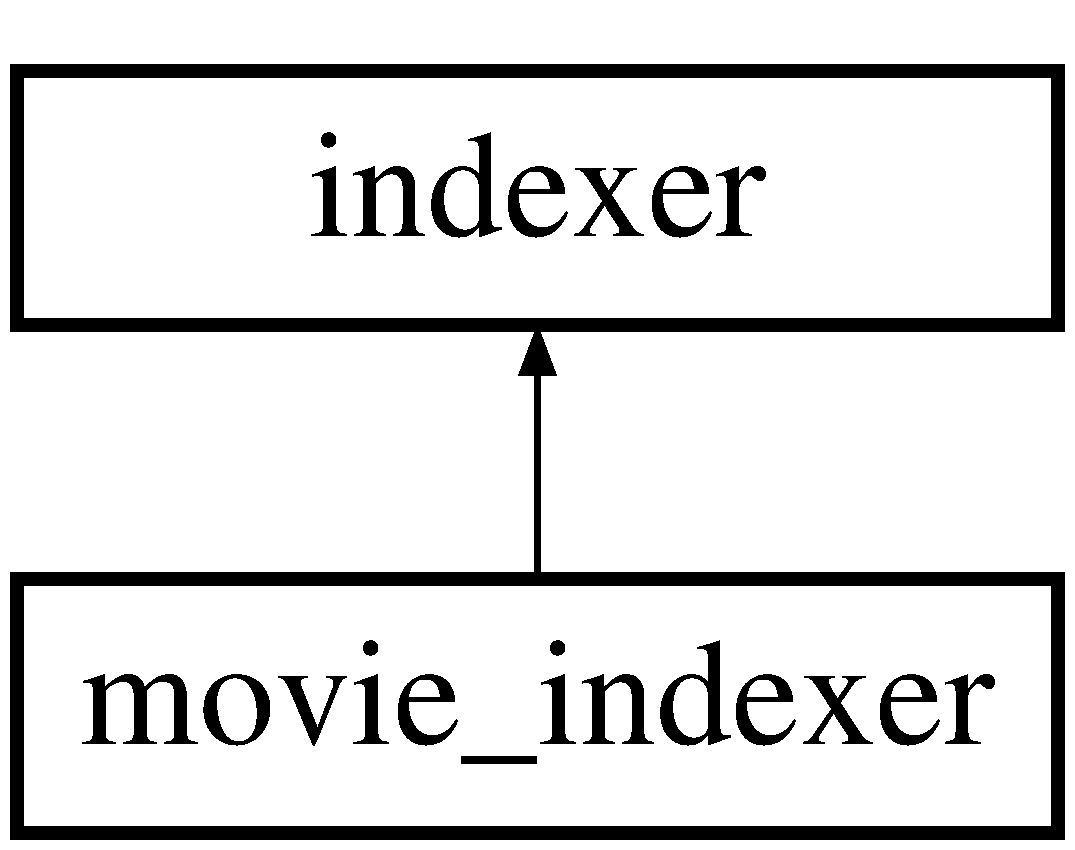
\includegraphics[height=2.000000cm]{classmovie__indexer}
\end{center}
\end{figure}
\subsection*{Public Member Functions}
\begin{DoxyCompactItemize}
\item 
\hyperlink{classmovie__indexer_a24fcbe6f81f28e9007202cd96df5e191}{movie\+\_\+indexer} ()
\begin{DoxyCompactList}\small\item\em a default constructor. \end{DoxyCompactList}\item 
vector$<$ \hyperlink{classmovie}{movie} $\ast$ $>$ \hyperlink{classmovie__indexer_a5b7aa1d935689ad1afbcfe2c877d3ae9}{operator\mbox{[}$\,$\mbox{]}} (string name)
\begin{DoxyCompactList}\small\item\em An operator\mbox{[}\mbox{]} overload. \end{DoxyCompactList}\item 
\hyperlink{classindex__item}{index\+\_\+item} $\ast$ \hyperlink{classmovie__indexer_aeaadd1ac660403a0f55122c6afea3acc}{operator\mbox{[}$\,$\mbox{]}} (int n)
\begin{DoxyCompactList}\small\item\em an operator\mbox{[}\mbox{]} overload. \end{DoxyCompactList}\end{DoxyCompactItemize}
\subsection*{Additional Inherited Members}


\subsection{Constructor \& Destructor Documentation}
\mbox{\Hypertarget{classmovie__indexer_a24fcbe6f81f28e9007202cd96df5e191}\label{classmovie__indexer_a24fcbe6f81f28e9007202cd96df5e191}} 
\index{movie\+\_\+indexer@{movie\+\_\+indexer}!movie\+\_\+indexer@{movie\+\_\+indexer}}
\index{movie\+\_\+indexer@{movie\+\_\+indexer}!movie\+\_\+indexer@{movie\+\_\+indexer}}
\subsubsection{\texorpdfstring{movie\+\_\+indexer()}{movie\_indexer()}}
{\footnotesize\ttfamily movie\+\_\+indexer\+::movie\+\_\+indexer (\begin{DoxyParamCaption}{ }\end{DoxyParamCaption})}



a default constructor. 

Initializes the indexer\textquotesingle{}s N to 0, normalized to false, and stpw to a stopwords (\char`\"{}stopwords.\+txt\char`\"{}). 

\subsection{Member Function Documentation}
\mbox{\Hypertarget{classmovie__indexer_a5b7aa1d935689ad1afbcfe2c877d3ae9}\label{classmovie__indexer_a5b7aa1d935689ad1afbcfe2c877d3ae9}} 
\index{movie\+\_\+indexer@{movie\+\_\+indexer}!operator\mbox{[}\mbox{]}@{operator[]}}
\index{operator\mbox{[}\mbox{]}@{operator[]}!movie\+\_\+indexer@{movie\+\_\+indexer}}
\subsubsection{\texorpdfstring{operator[]()}{operator[]()}\hspace{0.1cm}{\footnotesize\ttfamily [1/2]}}
{\footnotesize\ttfamily vector$<$ \hyperlink{classmovie}{movie} $\ast$ $>$ movie\+\_\+indexer\+::operator\mbox{[}$\,$\mbox{]} (\begin{DoxyParamCaption}\item[{string}]{name }\end{DoxyParamCaption})}



An operator\mbox{[}\mbox{]} overload. 


\begin{DoxyParams}{Parameters}
{\em name} & the name of the movies to return \\
\hline
\end{DoxyParams}
\begin{DoxyReturn}{Returns}
the document with filename name
\end{DoxyReturn}
Iterates through all items, and returns the movie with title name \mbox{\Hypertarget{classmovie__indexer_aeaadd1ac660403a0f55122c6afea3acc}\label{classmovie__indexer_aeaadd1ac660403a0f55122c6afea3acc}} 
\index{movie\+\_\+indexer@{movie\+\_\+indexer}!operator\mbox{[}\mbox{]}@{operator[]}}
\index{operator\mbox{[}\mbox{]}@{operator[]}!movie\+\_\+indexer@{movie\+\_\+indexer}}
\subsubsection{\texorpdfstring{operator[]()}{operator[]()}\hspace{0.1cm}{\footnotesize\ttfamily [2/2]}}
{\footnotesize\ttfamily \hyperlink{classindex__item}{index\+\_\+item} $\ast$ movie\+\_\+indexer\+::operator\mbox{[}$\,$\mbox{]} (\begin{DoxyParamCaption}\item[{int}]{n }\end{DoxyParamCaption})\hspace{0.3cm}{\ttfamily [virtual]}}



an operator\mbox{[}\mbox{]} overload. 


\begin{DoxyParams}{Parameters}
{\em n} & an int index. \\
\hline
\end{DoxyParams}
\begin{DoxyReturn}{Returns}
the movie at index n.
\end{DoxyReturn}
Gets the indexer\textquotesingle{}s n\textquotesingle{}th document. 

Reimplemented from \hyperlink{classindexer_ae71041fc84d94155473de60e4407d5cc}{indexer}.



The documentation for this class was generated from the following files\+:\begin{DoxyCompactItemize}
\item 
movie\+\_\+indexer.\+h\item 
movie\+\_\+indexer.\+cpp\end{DoxyCompactItemize}

\hypertarget{classmovie__tokenizer}{}\section{movie\+\_\+tokenizer Class Reference}
\label{classmovie__tokenizer}\index{movie\+\_\+tokenizer@{movie\+\_\+tokenizer}}
Inheritance diagram for movie\+\_\+tokenizer\+:\begin{figure}[H]
\begin{center}
\leavevmode
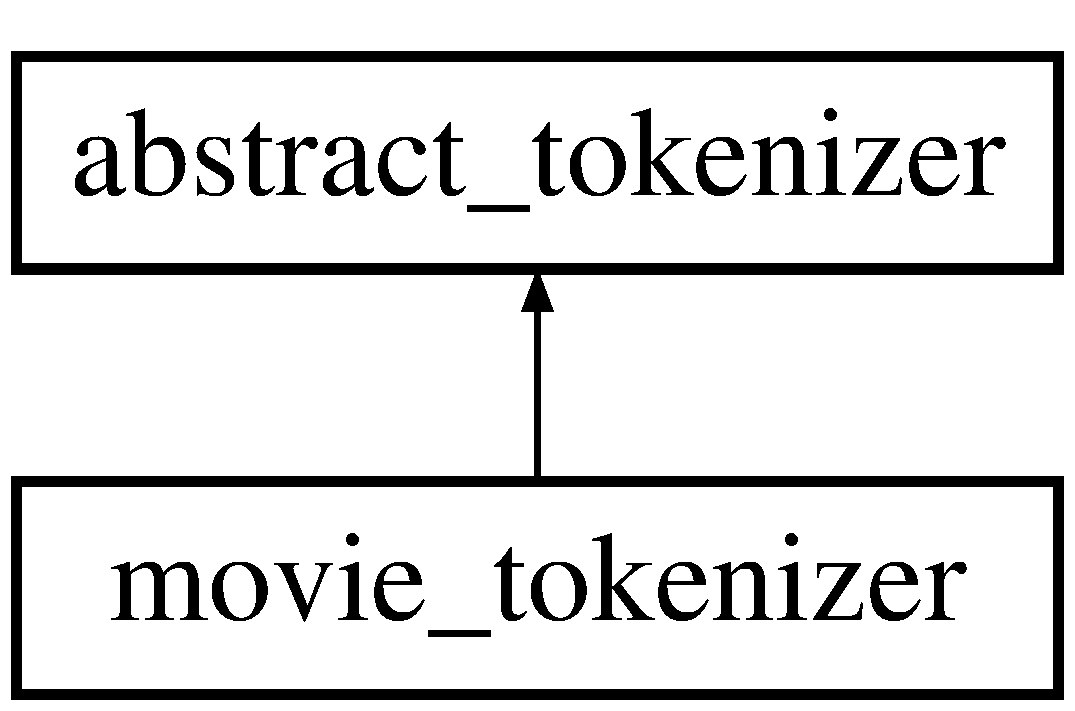
\includegraphics[height=2.000000cm]{classmovie__tokenizer}
\end{center}
\end{figure}
\subsection*{Public Member Functions}
\begin{DoxyCompactItemize}
\item 
\mbox{\Hypertarget{classmovie__tokenizer_af30c3fa452d1d99cb97d236494a5ea0c}\label{classmovie__tokenizer_af30c3fa452d1d99cb97d236494a5ea0c}} 
\hyperlink{classmovie__tokenizer_af30c3fa452d1d99cb97d236494a5ea0c}{movie\+\_\+tokenizer} ()
\begin{DoxyCompactList}\small\item\em A default constructor. \end{DoxyCompactList}\item 
vector$<$ \hyperlink{classmovie}{movie} $>$ \hyperlink{classmovie__tokenizer_a84002e6539255bfb4da76f0c86238c36}{movie\+\_\+tokenize} (string M\+E\+T\+A\+\_\+\+D\+A\+T\+A\+\_\+\+F\+I\+LE, string D\+E\+S\+C\+R\+I\+P\+T\+I\+O\+N\+\_\+\+F\+I\+LE)
\begin{DoxyCompactList}\small\item\em Reads two files and returns a vector of movies. \end{DoxyCompactList}\end{DoxyCompactItemize}


\subsection{Member Function Documentation}
\mbox{\Hypertarget{classmovie__tokenizer_a84002e6539255bfb4da76f0c86238c36}\label{classmovie__tokenizer_a84002e6539255bfb4da76f0c86238c36}} 
\index{movie\+\_\+tokenizer@{movie\+\_\+tokenizer}!movie\+\_\+tokenize@{movie\+\_\+tokenize}}
\index{movie\+\_\+tokenize@{movie\+\_\+tokenize}!movie\+\_\+tokenizer@{movie\+\_\+tokenizer}}
\subsubsection{\texorpdfstring{movie\+\_\+tokenize()}{movie\_tokenize()}}
{\footnotesize\ttfamily vector$<$ \hyperlink{classmovie}{movie} $>$ movie\+\_\+tokenizer\+::movie\+\_\+tokenize (\begin{DoxyParamCaption}\item[{string}]{M\+E\+T\+A\+\_\+\+D\+A\+T\+A\+\_\+\+F\+I\+LE,  }\item[{string}]{D\+E\+S\+C\+R\+I\+P\+T\+I\+O\+N\+\_\+\+F\+I\+LE }\end{DoxyParamCaption})}



Reads two files and returns a vector of movies. 


\begin{DoxyParams}{Parameters}
{\em M\+E\+T\+A\+\_\+\+D\+A\+T\+A\+\_\+\+F\+I\+LE} & The filename of the file containing the movie meta data. \\
\hline
{\em D\+E\+S\+C\+R\+I\+P\+T\+I\+O\+N\+\_\+\+F\+I\+LE} & The filename of the file containing the movie descriptions. \\
\hline
\end{DoxyParams}
\begin{DoxyReturn}{Returns}
All the movies that have descriptions in the the files.
\end{DoxyReturn}
This function reads all the available data in two files\+: The M\+E\+T\+A\+\_\+\+D\+A\+T\+A\+\_\+\+F\+I\+LE and the D\+E\+S\+C\+R\+I\+P\+T\+I\+O\+N\+\_\+\+F\+I\+LE It then associates the data contained in each by a common piece of data between the two\+: the Movie ID Then a vector of movies with descriptions is created and returned. 

The documentation for this class was generated from the following files\+:\begin{DoxyCompactItemize}
\item 
movie\+\_\+tokenizer.\+h\item 
movie\+\_\+tokenizer.\+cpp\end{DoxyCompactItemize}

\hypertarget{class_query___result}{}\section{Query\+\_\+\+Result Class Reference}
\label{class_query___result}\index{Query\+\_\+\+Result@{Query\+\_\+\+Result}}
\subsection*{Public Member Functions}
\begin{DoxyCompactItemize}
\item 
\hyperlink{class_query___result_aca6caea4d2be58145212fc22c56a5fab}{Query\+\_\+\+Result} ()
\begin{DoxyCompactList}\small\item\em The default constructor. \end{DoxyCompactList}\item 
\mbox{\Hypertarget{class_query___result_a12b2802d889af86623d0b1b646ca6854}\label{class_query___result_a12b2802d889af86623d0b1b646ca6854}} 
\hyperlink{class_query___result_a12b2802d889af86623d0b1b646ca6854}{$\sim$\+Query\+\_\+\+Result} ()
\begin{DoxyCompactList}\small\item\em The default destructor. \end{DoxyCompactList}\item 
const vector$<$ pair$<$ \hyperlink{classindex__item}{index\+\_\+item} $\ast$, double $>$ $>$ \& \hyperlink{class_query___result_a4ef5504013529a3b61b1d064ad75b348}{scorevector} ()
\begin{DoxyCompactList}\small\item\em An accessor for the score. \end{DoxyCompactList}\item 
void \hyperlink{class_query___result_a444ded4e65dab7222256ed6591ff78d9}{query} (\hyperlink{classindexer}{indexer} \&idx, string s)
\begin{DoxyCompactList}\small\item\em A function to apply a query and return a result. \end{DoxyCompactList}\item 
void \hyperlink{class_query___result_a5a3054d05f8768e724886d3cae6970c1}{print\+Doc\+Results} (\hyperlink{classdocument__indexer}{document\+\_\+indexer} \&idx, string s, int n=10)
\begin{DoxyCompactList}\small\item\em A function to print information about the documents found in indexer. \end{DoxyCompactList}\item 
vector$<$ \hyperlink{classindex__item}{index\+\_\+item} $\ast$ $>$ \hyperlink{class_query___result_a05014e96b4883c7ca78c7bd3b2e457d8}{get\+Top\+N\+Results} (int n, \hyperlink{classindex__item}{index\+\_\+item} $\ast$item\+To\+Filter=nullptr)
\begin{DoxyCompactList}\small\item\em A function to get the top n scores. \end{DoxyCompactList}\item 
string \hyperlink{class_query___result_a4729716b1a3d34c761a56d4d96ff906f}{generate\+Essay\+From\+Sentences} (int word\+Count) const
\begin{DoxyCompactList}\small\item\em A function to generate an essay from our queried sentences. \end{DoxyCompactList}\end{DoxyCompactItemize}


\subsection{Constructor \& Destructor Documentation}
\mbox{\Hypertarget{class_query___result_aca6caea4d2be58145212fc22c56a5fab}\label{class_query___result_aca6caea4d2be58145212fc22c56a5fab}} 
\index{Query\+\_\+\+Result@{Query\+\_\+\+Result}!Query\+\_\+\+Result@{Query\+\_\+\+Result}}
\index{Query\+\_\+\+Result@{Query\+\_\+\+Result}!Query\+\_\+\+Result@{Query\+\_\+\+Result}}
\subsubsection{\texorpdfstring{Query\+\_\+\+Result()}{Query\_Result()}}
{\footnotesize\ttfamily Query\+\_\+\+Result\+::\+Query\+\_\+\+Result (\begin{DoxyParamCaption}{ }\end{DoxyParamCaption})}



The default constructor. 

Is necessary for compilation. 

\subsection{Member Function Documentation}
\mbox{\Hypertarget{class_query___result_a4729716b1a3d34c761a56d4d96ff906f}\label{class_query___result_a4729716b1a3d34c761a56d4d96ff906f}} 
\index{Query\+\_\+\+Result@{Query\+\_\+\+Result}!generate\+Essay\+From\+Sentences@{generate\+Essay\+From\+Sentences}}
\index{generate\+Essay\+From\+Sentences@{generate\+Essay\+From\+Sentences}!Query\+\_\+\+Result@{Query\+\_\+\+Result}}
\subsubsection{\texorpdfstring{generate\+Essay\+From\+Sentences()}{generateEssayFromSentences()}}
{\footnotesize\ttfamily string Query\+\_\+\+Result\+::generate\+Essay\+From\+Sentences (\begin{DoxyParamCaption}\item[{int}]{word\+Count }\end{DoxyParamCaption}) const}



A function to generate an essay from our queried sentences. 


\begin{DoxyParams}{Parameters}
{\em word\+Count} & the maximum number of words for the essay \\
\hline
\end{DoxyParams}
\begin{DoxyReturn}{Returns}
the score
\end{DoxyReturn}
This function generates an essay from the contents of the score vector$<$pair$>$. The sentences that score contains are evaluated based on their word length to see if they are suitable given the requested number of words. If successful the sentence is placed in the chosen\+Sentences vector and then sorted by position. The \char`\"{}essay\char`\"{} is then returned as a string. \mbox{\Hypertarget{class_query___result_a05014e96b4883c7ca78c7bd3b2e457d8}\label{class_query___result_a05014e96b4883c7ca78c7bd3b2e457d8}} 
\index{Query\+\_\+\+Result@{Query\+\_\+\+Result}!get\+Top\+N\+Results@{get\+Top\+N\+Results}}
\index{get\+Top\+N\+Results@{get\+Top\+N\+Results}!Query\+\_\+\+Result@{Query\+\_\+\+Result}}
\subsubsection{\texorpdfstring{get\+Top\+N\+Results()}{getTopNResults()}}
{\footnotesize\ttfamily vector$<$ \hyperlink{classindex__item}{index\+\_\+item} $\ast$ $>$ Query\+\_\+\+Result\+::get\+Top\+N\+Results (\begin{DoxyParamCaption}\item[{int}]{n,  }\item[{\hyperlink{classindex__item}{index\+\_\+item} $\ast$}]{item\+To\+Filter = {\ttfamily nullptr} }\end{DoxyParamCaption})}



A function to get the top n scores. 


\begin{DoxyParams}{Parameters}
{\em n} & the top-\/n scores \\
\hline
\end{DoxyParams}
\begin{DoxyReturn}{Returns}
a vector of the top-\/n scores
\end{DoxyReturn}
This function gets the top N items in the score. \mbox{\Hypertarget{class_query___result_a5a3054d05f8768e724886d3cae6970c1}\label{class_query___result_a5a3054d05f8768e724886d3cae6970c1}} 
\index{Query\+\_\+\+Result@{Query\+\_\+\+Result}!print\+Doc\+Results@{print\+Doc\+Results}}
\index{print\+Doc\+Results@{print\+Doc\+Results}!Query\+\_\+\+Result@{Query\+\_\+\+Result}}
\subsubsection{\texorpdfstring{print\+Doc\+Results()}{printDocResults()}}
{\footnotesize\ttfamily void Query\+\_\+\+Result\+::print\+Doc\+Results (\begin{DoxyParamCaption}\item[{\hyperlink{classdocument__indexer}{document\+\_\+indexer} \&}]{idx,  }\item[{string}]{s,  }\item[{int}]{n = {\ttfamily 10} }\end{DoxyParamCaption})}



A function to print information about the documents found in indexer. 


\begin{DoxyParams}{Parameters}
{\em idx} & the indexer to be used \\
\hline
{\em s} & the given query \\
\hline
{\em n} & the top-\/n documents to be returned\\
\hline
\end{DoxyParams}
This function prints the items contained in the index as documents. Printing out the name of the document and its score. \mbox{\Hypertarget{class_query___result_a444ded4e65dab7222256ed6591ff78d9}\label{class_query___result_a444ded4e65dab7222256ed6591ff78d9}} 
\index{Query\+\_\+\+Result@{Query\+\_\+\+Result}!query@{query}}
\index{query@{query}!Query\+\_\+\+Result@{Query\+\_\+\+Result}}
\subsubsection{\texorpdfstring{query()}{query()}}
{\footnotesize\ttfamily void Query\+\_\+\+Result\+::query (\begin{DoxyParamCaption}\item[{\hyperlink{classindexer}{indexer} \&}]{idx,  }\item[{string}]{s }\end{DoxyParamCaption})}



A function to apply a query and return a result. 


\begin{DoxyTemplParams}{Template Parameters}
{\em size} & the size of indexer. \\
\hline
\end{DoxyTemplParams}

\begin{DoxyParams}{Parameters}
{\em idx} & The indexer on which the query will be applied \\
\hline
{\em s} & A string that is to be searched for in the indexer. \\
\hline
{\em n} & an optional int to delimit the amount of results printed out, default is 10. \\
\hline
\end{DoxyParams}
\begin{DoxyReturn}{Returns}
the score
\end{DoxyReturn}
This function first checks if the indexer is normalized. If it is not, throw an error. It then goes through every document in the indexer, and calculates the weights per document. Using the weights, it calculates every document\textquotesingle{}s score. It the prints out the n top scores, and returns all scores. \mbox{\Hypertarget{class_query___result_a4ef5504013529a3b61b1d064ad75b348}\label{class_query___result_a4ef5504013529a3b61b1d064ad75b348}} 
\index{Query\+\_\+\+Result@{Query\+\_\+\+Result}!scorevector@{scorevector}}
\index{scorevector@{scorevector}!Query\+\_\+\+Result@{Query\+\_\+\+Result}}
\subsubsection{\texorpdfstring{scorevector()}{scorevector()}}
{\footnotesize\ttfamily const vector$<$ pair$<$ \hyperlink{classindex__item}{index\+\_\+item} $\ast$, double $>$ $>$ \& Query\+\_\+\+Result\+::scorevector (\begin{DoxyParamCaption}{ }\end{DoxyParamCaption})}



An accessor for the score. 

\begin{DoxyReturn}{Returns}
The score of the query result. 
\end{DoxyReturn}


The documentation for this class was generated from the following files\+:\begin{DoxyCompactItemize}
\item 
Query\+\_\+\+Result.\+h\item 
query\+\_\+result.\+cpp\end{DoxyCompactItemize}

\hypertarget{classsentence}{}\section{sentence Class Reference}
\label{classsentence}\index{sentence@{sentence}}
Inheritance diagram for sentence\+:\begin{figure}[H]
\begin{center}
\leavevmode
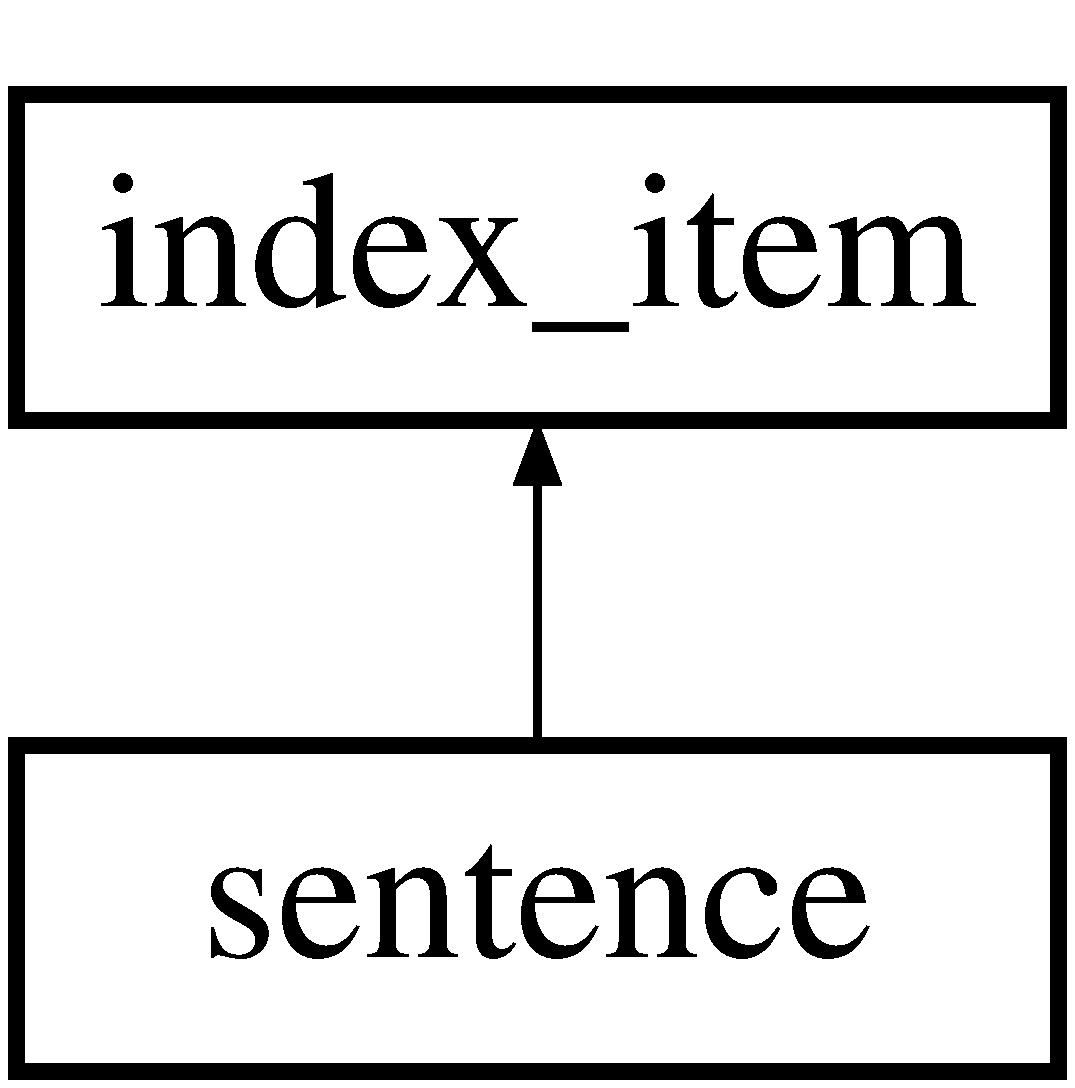
\includegraphics[height=2.000000cm]{classsentence}
\end{center}
\end{figure}
\subsection*{Public Member Functions}
\begin{DoxyCompactItemize}
\item 
\hyperlink{classsentence_a458e5abe0d27f8972771153e72667673}{sentence} ()
\begin{DoxyCompactList}\small\item\em A default constructor. \end{DoxyCompactList}\item 
\hyperlink{classsentence_a39e99adb96c8de8aeff00c0657248f9e}{sentence} (string s, int p, int doc\+Num)
\begin{DoxyCompactList}\small\item\em Another constructor. \end{DoxyCompactList}\item 
\mbox{\Hypertarget{classsentence_affdf5776454bd6796aac043ff8b9630e}\label{classsentence_affdf5776454bd6796aac043ff8b9630e}} 
\hyperlink{classsentence_affdf5776454bd6796aac043ff8b9630e}{$\sim$sentence} ()
\begin{DoxyCompactList}\small\item\em The default destructor. \end{DoxyCompactList}\item 
int \hyperlink{classsentence_ad4786351fceabfd06ca10b7766d516b3}{get\+Pos} () const
\begin{DoxyCompactList}\small\item\em An accessor for the sentence\textquotesingle{}s position in a document. \end{DoxyCompactList}\item 
int \hyperlink{classsentence_a6b8b9942e1a30a75ca2308d6b71fb24d}{get\+Parent\+Doc\+Num} () const
\begin{DoxyCompactList}\small\item\em An accessor for the sentence\textquotesingle{}s document number. \end{DoxyCompactList}\item 
bool \hyperlink{classsentence_ae4cbc4603c414be42f68131e243e1bed}{operator$<$} (const \hyperlink{classsentence}{sentence} \&other)
\begin{DoxyCompactList}\small\item\em a default $<$ operator \end{DoxyCompactList}\end{DoxyCompactItemize}
\subsection*{Additional Inherited Members}


\subsection{Constructor \& Destructor Documentation}
\mbox{\Hypertarget{classsentence_a458e5abe0d27f8972771153e72667673}\label{classsentence_a458e5abe0d27f8972771153e72667673}} 
\index{sentence@{sentence}!sentence@{sentence}}
\index{sentence@{sentence}!sentence@{sentence}}
\subsubsection{\texorpdfstring{sentence()}{sentence()}\hspace{0.1cm}{\footnotesize\ttfamily [1/2]}}
{\footnotesize\ttfamily sentence\+::sentence (\begin{DoxyParamCaption}{ }\end{DoxyParamCaption})}



A default constructor. 

The default constructor sets the content to \char`\"{}\char`\"{}, the size to 0, and the pos to 0 \mbox{\Hypertarget{classsentence_a39e99adb96c8de8aeff00c0657248f9e}\label{classsentence_a39e99adb96c8de8aeff00c0657248f9e}} 
\index{sentence@{sentence}!sentence@{sentence}}
\index{sentence@{sentence}!sentence@{sentence}}
\subsubsection{\texorpdfstring{sentence()}{sentence()}\hspace{0.1cm}{\footnotesize\ttfamily [2/2]}}
{\footnotesize\ttfamily sentence\+::sentence (\begin{DoxyParamCaption}\item[{string}]{s,  }\item[{int}]{p,  }\item[{int}]{doc\+Num }\end{DoxyParamCaption})}



Another constructor. 


\begin{DoxyParams}{Parameters}
{\em s} & content of the sentence to be constructed. \\
\hline
{\em p} & the position of the sentence in the string. \\
\hline
{\em doc\+Num} & the number of the document from which the string originates.\\
\hline
\end{DoxyParams}
The constructor takes a string s, and sets the sentence\textquotesingle{}s content to that string It also takes int p, and sets the sentence\textquotesingle{}s supposed position in a document to that int It then splits the content of the sentence based on white spaces and sets the size of the sentence to the number of tokens that were split 

\subsection{Member Function Documentation}
\mbox{\Hypertarget{classsentence_a6b8b9942e1a30a75ca2308d6b71fb24d}\label{classsentence_a6b8b9942e1a30a75ca2308d6b71fb24d}} 
\index{sentence@{sentence}!get\+Parent\+Doc\+Num@{get\+Parent\+Doc\+Num}}
\index{get\+Parent\+Doc\+Num@{get\+Parent\+Doc\+Num}!sentence@{sentence}}
\subsubsection{\texorpdfstring{get\+Parent\+Doc\+Num()}{getParentDocNum()}}
{\footnotesize\ttfamily int sentence\+::get\+Parent\+Doc\+Num (\begin{DoxyParamCaption}{ }\end{DoxyParamCaption}) const}



An accessor for the sentence\textquotesingle{}s document number. 

\begin{DoxyReturn}{Returns}
An int, the document number.
\end{DoxyReturn}
This accessor returns the sentence\textquotesingle{}s parent document number \mbox{\Hypertarget{classsentence_ad4786351fceabfd06ca10b7766d516b3}\label{classsentence_ad4786351fceabfd06ca10b7766d516b3}} 
\index{sentence@{sentence}!get\+Pos@{get\+Pos}}
\index{get\+Pos@{get\+Pos}!sentence@{sentence}}
\subsubsection{\texorpdfstring{get\+Pos()}{getPos()}}
{\footnotesize\ttfamily int sentence\+::get\+Pos (\begin{DoxyParamCaption}{ }\end{DoxyParamCaption}) const}



An accessor for the sentence\textquotesingle{}s position in a document. 

\begin{DoxyReturn}{Returns}
An int, the starting position of the sentence.
\end{DoxyReturn}
This accessor returns the sentence\textquotesingle{}s position in the document \mbox{\Hypertarget{classsentence_ae4cbc4603c414be42f68131e243e1bed}\label{classsentence_ae4cbc4603c414be42f68131e243e1bed}} 
\index{sentence@{sentence}!operator$<$@{operator$<$}}
\index{operator$<$@{operator$<$}!sentence@{sentence}}
\subsubsection{\texorpdfstring{operator$<$()}{operator<()}}
{\footnotesize\ttfamily bool sentence\+::operator$<$ (\begin{DoxyParamCaption}\item[{const \hyperlink{classsentence}{sentence} \&}]{other }\end{DoxyParamCaption})}



a default $<$ operator 


\begin{DoxyParams}{Parameters}
{\em other} & a sentence to compare {\itshape this} to \\
\hline
\end{DoxyParams}
\begin{DoxyReturn}{Returns}
a boolean. Whether other is greater than {\itshape this}
\end{DoxyReturn}
First, orders sentences by document number T\+Hen, orders them by their position in the document 

The documentation for this class was generated from the following files\+:\begin{DoxyCompactItemize}
\item 
sentence.\+h\item 
sentence.\+cpp\end{DoxyCompactItemize}

\hypertarget{classsentence__tokenizer}{}\section{sentence\+\_\+tokenizer Class Reference}
\label{classsentence__tokenizer}\index{sentence\+\_\+tokenizer@{sentence\+\_\+tokenizer}}
Inheritance diagram for sentence\+\_\+tokenizer\+:\begin{figure}[H]
\begin{center}
\leavevmode
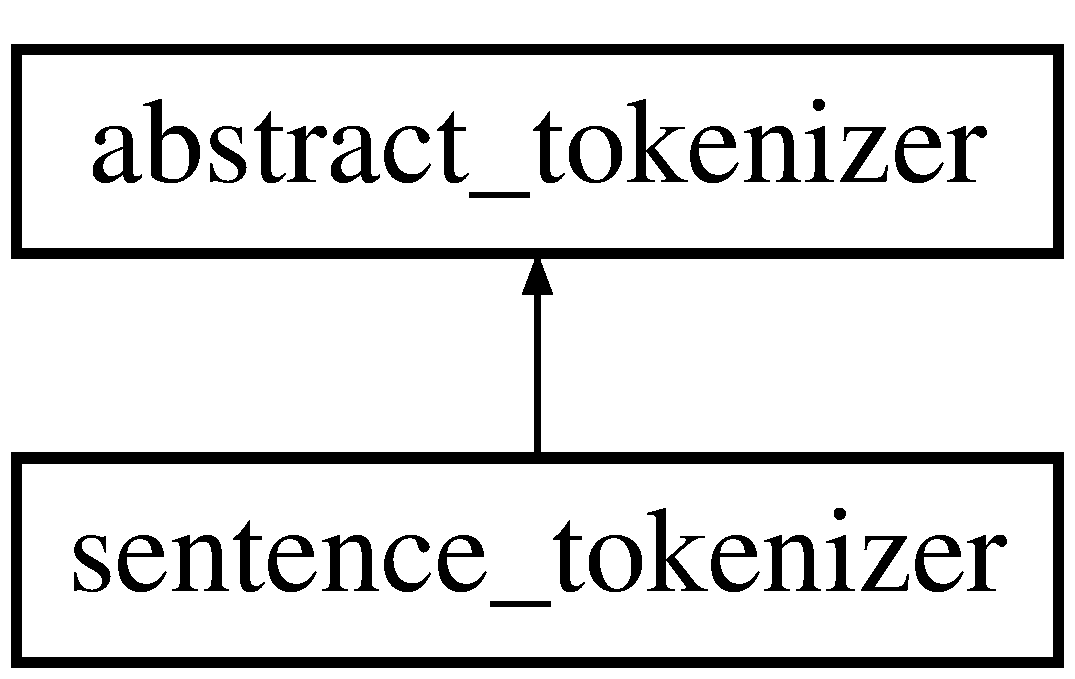
\includegraphics[height=2.000000cm]{classsentence__tokenizer}
\end{center}
\end{figure}
\subsection*{Public Member Functions}
\begin{DoxyCompactItemize}
\item 
\hyperlink{classsentence__tokenizer_aa36679bc4afb2788d5c81fcee4ab9e0b}{sentence\+\_\+tokenizer} ()
\begin{DoxyCompactList}\small\item\em A default constructor. \end{DoxyCompactList}\item 
\mbox{\Hypertarget{classsentence__tokenizer_ac15a8df6ebb233288866e8d692e514c8}\label{classsentence__tokenizer_ac15a8df6ebb233288866e8d692e514c8}} 
\hyperlink{classsentence__tokenizer_ac15a8df6ebb233288866e8d692e514c8}{$\sim$sentence\+\_\+tokenizer} ()
\begin{DoxyCompactList}\small\item\em A default destructor. \end{DoxyCompactList}\item 
vector$<$ \hyperlink{classsentence}{sentence} $>$ \hyperlink{classsentence__tokenizer_ab394b821c6d32d41ae07ae84a0d1b5a6}{sentence\+\_\+tokenize} (const string \&s, int doc\+Num)
\begin{DoxyCompactList}\small\item\em A method to break down a string into a set of strings. \end{DoxyCompactList}\item 
bool \hyperlink{classsentence__tokenizer_accdc817790cdb696912ec8076701f8a9}{is\+\_\+end} (const char \&c)
\begin{DoxyCompactList}\small\item\em A method to check if a char is either \char`\"{}?\char`\"{} OR \char`\"{}.\char`\"{} OR \char`\"{}!\char`\"{}. \end{DoxyCompactList}\item 
bool \hyperlink{classsentence__tokenizer_a2f86e3437eb3a948b5ee309ce04d0029}{is\+Abbreviation} (const string \&first, const string \&second)
\begin{DoxyCompactList}\small\item\em A method to check if a string is an abbreviation. \end{DoxyCompactList}\end{DoxyCompactItemize}


\subsection{Constructor \& Destructor Documentation}
\mbox{\Hypertarget{classsentence__tokenizer_aa36679bc4afb2788d5c81fcee4ab9e0b}\label{classsentence__tokenizer_aa36679bc4afb2788d5c81fcee4ab9e0b}} 
\index{sentence\+\_\+tokenizer@{sentence\+\_\+tokenizer}!sentence\+\_\+tokenizer@{sentence\+\_\+tokenizer}}
\index{sentence\+\_\+tokenizer@{sentence\+\_\+tokenizer}!sentence\+\_\+tokenizer@{sentence\+\_\+tokenizer}}
\subsubsection{\texorpdfstring{sentence\+\_\+tokenizer()}{sentence\_tokenizer()}}
{\footnotesize\ttfamily sentence\+\_\+tokenizer\+::sentence\+\_\+tokenizer (\begin{DoxyParamCaption}{ }\end{DoxyParamCaption})}



A default constructor. 

The default constructor. 

\subsection{Member Function Documentation}
\mbox{\Hypertarget{classsentence__tokenizer_accdc817790cdb696912ec8076701f8a9}\label{classsentence__tokenizer_accdc817790cdb696912ec8076701f8a9}} 
\index{sentence\+\_\+tokenizer@{sentence\+\_\+tokenizer}!is\+\_\+end@{is\+\_\+end}}
\index{is\+\_\+end@{is\+\_\+end}!sentence\+\_\+tokenizer@{sentence\+\_\+tokenizer}}
\subsubsection{\texorpdfstring{is\+\_\+end()}{is\_end()}}
{\footnotesize\ttfamily bool sentence\+\_\+tokenizer\+::is\+\_\+end (\begin{DoxyParamCaption}\item[{const char \&}]{c }\end{DoxyParamCaption})}



A method to check if a char is either \char`\"{}?\char`\"{} OR \char`\"{}.\char`\"{} OR \char`\"{}!\char`\"{}. 


\begin{DoxyParams}{Parameters}
{\em c} & the char to be tested. \\
\hline
\end{DoxyParams}
\begin{DoxyReturn}{Returns}
a bool\+: the truth value that is determined by testing the char c.
\end{DoxyReturn}
Tests a char input to see whether it matches certain characters. \mbox{\Hypertarget{classsentence__tokenizer_a2f86e3437eb3a948b5ee309ce04d0029}\label{classsentence__tokenizer_a2f86e3437eb3a948b5ee309ce04d0029}} 
\index{sentence\+\_\+tokenizer@{sentence\+\_\+tokenizer}!is\+Abbreviation@{is\+Abbreviation}}
\index{is\+Abbreviation@{is\+Abbreviation}!sentence\+\_\+tokenizer@{sentence\+\_\+tokenizer}}
\subsubsection{\texorpdfstring{is\+Abbreviation()}{isAbbreviation()}}
{\footnotesize\ttfamily bool sentence\+\_\+tokenizer\+::is\+Abbreviation (\begin{DoxyParamCaption}\item[{const string \&}]{first,  }\item[{const string \&}]{second }\end{DoxyParamCaption})}



A method to check if a string is an abbreviation. 


\begin{DoxyParams}{Parameters}
{\em first} & the string to be tested. \\
\hline
{\em second} & This is the string which appears after first, it is used in the detection of abbreviations \\
\hline
\end{DoxyParams}
\begin{DoxyReturn}{Returns}
a bool\+: the truth value that is determined by testing the string first.
\end{DoxyReturn}
Tests a string (first) to determine if it is an abbreviation of a word or not. Three checks are performed\+: If the string does not end in \char`\"{}.\char`\"{} it is not an abbreviation If the string following the first string (second) is in lower case then first must be an abbreviation. If first and second are in uppercase and the length of first is less than or equal to 4 we assume it is an abbreviation of a title. \mbox{\Hypertarget{classsentence__tokenizer_ab394b821c6d32d41ae07ae84a0d1b5a6}\label{classsentence__tokenizer_ab394b821c6d32d41ae07ae84a0d1b5a6}} 
\index{sentence\+\_\+tokenizer@{sentence\+\_\+tokenizer}!sentence\+\_\+tokenize@{sentence\+\_\+tokenize}}
\index{sentence\+\_\+tokenize@{sentence\+\_\+tokenize}!sentence\+\_\+tokenizer@{sentence\+\_\+tokenizer}}
\subsubsection{\texorpdfstring{sentence\+\_\+tokenize()}{sentence\_tokenize()}}
{\footnotesize\ttfamily vector$<$ \hyperlink{classsentence}{sentence} $>$ sentence\+\_\+tokenizer\+::sentence\+\_\+tokenize (\begin{DoxyParamCaption}\item[{const string \&}]{s,  }\item[{int}]{doc\+Num }\end{DoxyParamCaption})}



A method to break down a string into a set of strings. 


\begin{DoxyParams}{Parameters}
{\em s} & the string to be broken down. \\
\hline
{\em doc\+Num} & the doc number of the string s (parent\+Doc\+Num of sentence) \\
\hline
\end{DoxyParams}
\begin{DoxyReturn}{Returns}
a vector$<$string$>$\+: the set of strings that make up s, split into sentences based on punctuation and grammar.
\end{DoxyReturn}
The sentence\+\_\+tokenize method takes a string s, and first breaks it into tokens by splitting words by whitespace. It then takes every string in the vector, and begins adding them together to form a sentence. If the end of a sentence is detected. We store what is currently on the accumulator and reset the accumulator We continue iterating until we have exhausted all the tokens. Finally, it returns the new vector of sentences. 

The documentation for this class was generated from the following files\+:\begin{DoxyCompactItemize}
\item 
sentence\+\_\+tokenizer.\+h\item 
sentence\+\_\+tokenizer.\+cpp\end{DoxyCompactItemize}

\hypertarget{classstopwords}{}\section{stopwords Class Reference}
\label{classstopwords}\index{stopwords@{stopwords}}
\subsection*{Public Member Functions}
\begin{DoxyCompactItemize}
\item 
\hyperlink{classstopwords_ae07cdf9173446ac3ff166c26ba7f05d4}{stopwords} ()
\begin{DoxyCompactList}\small\item\em A default constructor. \end{DoxyCompactList}\item 
\mbox{\Hypertarget{classstopwords_acc1fd23d272a96a69860f185360df992}\label{classstopwords_acc1fd23d272a96a69860f185360df992}} 
\hyperlink{classstopwords_acc1fd23d272a96a69860f185360df992}{$\sim$stopwords} ()
\begin{DoxyCompactList}\small\item\em A default destructor. \end{DoxyCompactList}\item 
\hyperlink{classstopwords_a726865f116a88b84c2239e80a1fb872a}{stopwords} (string filename)
\begin{DoxyCompactList}\small\item\em Anoter constructor. \end{DoxyCompactList}\item 
bool \hyperlink{classstopwords_a7e237ef49803d27b80d5efcca17f53b3}{operator()} (string word)
\begin{DoxyCompactList}\small\item\em an operator() overlead. \end{DoxyCompactList}\end{DoxyCompactItemize}


\subsection{Constructor \& Destructor Documentation}
\mbox{\Hypertarget{classstopwords_ae07cdf9173446ac3ff166c26ba7f05d4}\label{classstopwords_ae07cdf9173446ac3ff166c26ba7f05d4}} 
\index{stopwords@{stopwords}!stopwords@{stopwords}}
\index{stopwords@{stopwords}!stopwords@{stopwords}}
\subsubsection{\texorpdfstring{stopwords()}{stopwords()}\hspace{0.1cm}{\footnotesize\ttfamily [1/2]}}
{\footnotesize\ttfamily stopwords\+::stopwords (\begin{DoxyParamCaption}{ }\end{DoxyParamCaption})}



A default constructor. 

The default constructor does nothing in this case, since we have no use for an empty stopwords object. \mbox{\Hypertarget{classstopwords_a726865f116a88b84c2239e80a1fb872a}\label{classstopwords_a726865f116a88b84c2239e80a1fb872a}} 
\index{stopwords@{stopwords}!stopwords@{stopwords}}
\index{stopwords@{stopwords}!stopwords@{stopwords}}
\subsubsection{\texorpdfstring{stopwords()}{stopwords()}\hspace{0.1cm}{\footnotesize\ttfamily [2/2]}}
{\footnotesize\ttfamily stopwords\+::stopwords (\begin{DoxyParamCaption}\item[{string}]{fname }\end{DoxyParamCaption})}



Anoter constructor. 


\begin{DoxyParams}{Parameters}
{\em filename} & the filename of the stopwords to be constructed.\\
\hline
\end{DoxyParams}
The other constructor takes a string fname and sets it as its filename. It then creates a filestream from the filename, and reads every word in the filestream into the stopword vector. 

\subsection{Member Function Documentation}
\mbox{\Hypertarget{classstopwords_a7e237ef49803d27b80d5efcca17f53b3}\label{classstopwords_a7e237ef49803d27b80d5efcca17f53b3}} 
\index{stopwords@{stopwords}!operator()@{operator()}}
\index{operator()@{operator()}!stopwords@{stopwords}}
\subsubsection{\texorpdfstring{operator()()}{operator()()}}
{\footnotesize\ttfamily bool stopwords\+::operator() (\begin{DoxyParamCaption}\item[{string}]{word }\end{DoxyParamCaption})}



an operator() overlead. 


\begin{DoxyParams}{Parameters}
{\em word} & the work to check if it is a stopword or not. \\
\hline
\end{DoxyParams}
\begin{DoxyReturn}{Returns}
a boolean\+: whether or not the word input is a stopword.
\end{DoxyReturn}
The overloaded operator() takes a word, and returns true if the work is in the stopword vector. Else, it returns false; 

The documentation for this class was generated from the following files\+:\begin{DoxyCompactItemize}
\item 
stopwords.\+h\item 
stopwords.\+cpp\end{DoxyCompactItemize}

\hypertarget{classword__tokenizer}{}\section{word\+\_\+tokenizer Class Reference}
\label{classword__tokenizer}\index{word\+\_\+tokenizer@{word\+\_\+tokenizer}}
Inheritance diagram for word\+\_\+tokenizer\+:\begin{figure}[H]
\begin{center}
\leavevmode
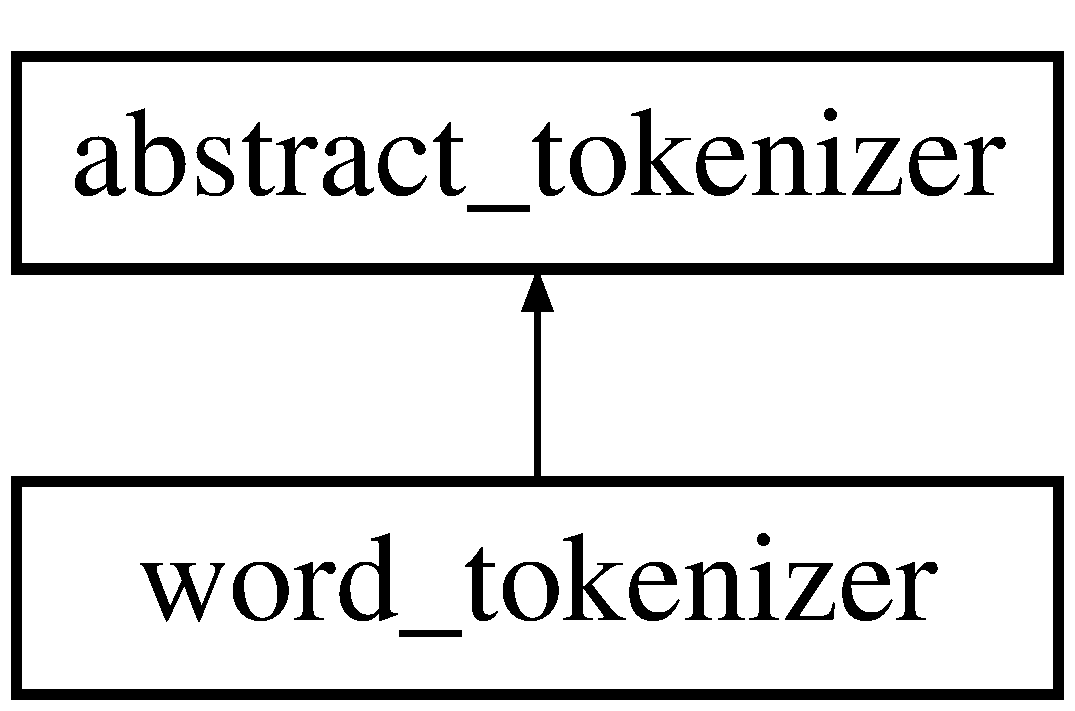
\includegraphics[height=2.000000cm]{classword__tokenizer}
\end{center}
\end{figure}
\subsection*{Public Member Functions}
\begin{DoxyCompactItemize}
\item 
\hyperlink{classword__tokenizer_a30887805b70d364fb6fde6cdd814c16a}{word\+\_\+tokenizer} ()
\begin{DoxyCompactList}\small\item\em A default constructor. \end{DoxyCompactList}\item 
\mbox{\Hypertarget{classword__tokenizer_a19a17890aac719ba8cb1459713f5a96e}\label{classword__tokenizer_a19a17890aac719ba8cb1459713f5a96e}} 
\hyperlink{classword__tokenizer_a19a17890aac719ba8cb1459713f5a96e}{$\sim$word\+\_\+tokenizer} ()
\begin{DoxyCompactList}\small\item\em A default destructor. \end{DoxyCompactList}\item 
vector$<$ string $>$ \hyperlink{classword__tokenizer_a4a77b2c08a636c15935a5c9dbd0d1d4f}{word\+\_\+tokenize} (string s)
\begin{DoxyCompactList}\small\item\em A method to break down a string into a set of strings. \end{DoxyCompactList}\end{DoxyCompactItemize}


\subsection{Constructor \& Destructor Documentation}
\mbox{\Hypertarget{classword__tokenizer_a30887805b70d364fb6fde6cdd814c16a}\label{classword__tokenizer_a30887805b70d364fb6fde6cdd814c16a}} 
\index{word\+\_\+tokenizer@{word\+\_\+tokenizer}!word\+\_\+tokenizer@{word\+\_\+tokenizer}}
\index{word\+\_\+tokenizer@{word\+\_\+tokenizer}!word\+\_\+tokenizer@{word\+\_\+tokenizer}}
\subsubsection{\texorpdfstring{word\+\_\+tokenizer()}{word\_tokenizer()}}
{\footnotesize\ttfamily word\+\_\+tokenizer\+::word\+\_\+tokenizer (\begin{DoxyParamCaption}{ }\end{DoxyParamCaption})}



A default constructor. 

Is necessary for compilation. 

\subsection{Member Function Documentation}
\mbox{\Hypertarget{classword__tokenizer_a4a77b2c08a636c15935a5c9dbd0d1d4f}\label{classword__tokenizer_a4a77b2c08a636c15935a5c9dbd0d1d4f}} 
\index{word\+\_\+tokenizer@{word\+\_\+tokenizer}!word\+\_\+tokenize@{word\+\_\+tokenize}}
\index{word\+\_\+tokenize@{word\+\_\+tokenize}!word\+\_\+tokenizer@{word\+\_\+tokenizer}}
\subsubsection{\texorpdfstring{word\+\_\+tokenize()}{word\_tokenize()}}
{\footnotesize\ttfamily vector$<$ string $>$ word\+\_\+tokenizer\+::word\+\_\+tokenize (\begin{DoxyParamCaption}\item[{string}]{s }\end{DoxyParamCaption})}



A method to break down a string into a set of strings. 


\begin{DoxyParams}{Parameters}
{\em s} & the string to be broken down. \\
\hline
\end{DoxyParams}
\begin{DoxyReturn}{Returns}
a vector$<$string$>$\+: the set of strings that make up s, minus whitespaces and punctuation.
\end{DoxyReturn}
The word\+\_\+tokenize method takes a string s, and first breaks it into an vector by dividing words by whitespace. It then takes every string in the vector, makes it lowercase and removes any punctuation. (i.\+e. \textquotesingle{}i-\/e.\+F\textquotesingle{} would become \textquotesingle{}ief\textquotesingle{}). It then adds the new string to a new vector. Finally, it returns the new vector of lowercase words with no punctuation. 

The documentation for this class was generated from the following files\+:\begin{DoxyCompactItemize}
\item 
word\+\_\+tokenizer.\+h\item 
word\+\_\+tokenizer.\+cpp\end{DoxyCompactItemize}

%--- End generated contents ---

% Index
\backmatter
\newpage
\phantomsection
\clearemptydoublepage
\addcontentsline{toc}{chapter}{Index}
\printindex

\end{document}
